\documentclass[11pt,a4paper]{article}

 \usepackage[utf8]{inputenc}
\usepackage[parfill]{parskip}  
\usepackage[a4paper, width=14cm, left=3.5cm]{geometry}
\usepackage{graphicx}
\usepackage{amssymb}
\usepackage{amsmath}
\usepackage{epstopdf}
\usepackage{rail}
\usepackage{ulem}
\usepackage{color}
\usepackage{xcolor}
\usepackage{makeidx}
\usepackage{mathtools}
\usepackage{multirow}
\usepackage{tabularx}
\usepackage{longtable}
\usepackage{tabu}
\usepackage{microtype}
\usepackage[style=numeric,sorting=nty,backend=biber]{biblatex}
\addbibresource{XMLPersistenceMapping.bib}
\DeclareFieldFormat{title}{{\itshape #1}}

%\setlength{\textwidth}{6.5in}

 % macro for \addtodo{todo} entries addition
 \newcommand{\addtodo}[1]{\textcolor{red}{[To do: #1]}\index{TODO: #1}}

\usepackage{minted}

\DeclareGraphicsRule{.tif}{png}{.png}{`convert #1 `dirname #1`/`basename #1 .tif`.png}

\usepackage[colorlinks=true, pdfstartview=FitV, linkcolor=blue, 
            citecolor=blue, urlcolor=blue]{hyperref}
            
\railoptions{ac}
\railoptions{i}
\railoptions{h}
%\railoptions{-h}

\railalias{quote}{'}
\railalias{dquote}{"}
\railalias{cr}{\char"5C\char"5C}
\railalias{featureNsPrefix}{{\color{blue} featureNsPrefix}}
\railalias{featureName}{{\color{blue} feature$\rhd$name}}
\railalias{featureWrapperName}{{\color{blue} feature$\rhd$wrapperName}}

\railalias{classifierNsPrefix}{{\color{blue} classifierNsPrefix}}
\railalias{classifierName}{{\color{blue} classifier$\rhd$name}}
\railalias{classifierWrapperName}{{\color{blue} classifier$\rhd$wrapperName}}
\railalias{targetURI}{{\color{blue} targetURI}}
\railalias{value}{{\color{blue} value}}
\railalias{classifierNameSuffix}{{\color{blue} suffix}}
\railalias{classifierWrapperNameSuffix}{{\color{blue} wrapperSuffix}}

\railalias{nsURI}{{\color{blue} nsURI}}
\railalias{nsPrefix}{{\color{blue} nsPrefix}}
\railalias{minOccurs}{{\color{blue} minOccurs}}
\railalias{maxOccurs}{{\color{blue} maxOccurs}}
\railalias{zero}{{\color{blue} 0}}
\railalias{one}{{\color{blue} 1}}


\railterm{quote,dquote,cr,featureNsPrefix,featureName,featureWrapperName,classifierNsPrefix,classifierName,classifierWrapperName,classifierWrapperNameSuffix,targetURI,value,classifierNameSuffix,nsURI,nsPrefix,minOccurs,maxOccurs,zero,one}

\railtermfont{\small\ttfamily\upshape}
\railnontermfont{\small\rmfamily\itshape\color{blue}}
\setlength\railboxskip{16pt}
\setlength\railboxheight{12pt}
\setlength\railovalspace{6pt}
\setlength\railframespace{5pt}
\setlength\railjoinsize{8pt}

\makeindex
%\includeonly{Chapter1}



\newtheorem{theorem}{Theorem}
\newtheorem{corollary}[theorem]{Corollary}
\newtheorem{definition}{Definition}
\newtheorem{lemma}{Lemma}
\newtheorem{exercise}{Exercise}
\newtheorem{remark}{Remark}
\newtheorem{example}{Example}
\newtheorem{warning}{Warning}

\def\grad{ \mbox{grad}}
\def\curl{ \mbox{curl}}
\def\div{ \mbox{div}}
\def\U{\ensuremath {\cal U}}
\def\S{\ensuremath {\cal S}}
\def\V{\ensuremath {\cal V}}
\def\R{\ensuremath {\cal R}}
\def\tr{\ensuremath {\mbox{tr}}}




% ------------------- Title and Author -----------------------------
\title{Specification of Ecore to XML Persistence Mapping}
\author{%
	\large
%	\textsc{Mark Br\"orkens$^1$, Yue Ma$^2$, Stephan Eberle$^2$, Bernhard Weichel$^3$} \\[2mm]
%	\normalsize	$^1$itemis AG \\
%	\normalsize       $^2$itemis France SAS\\
%	\normalsize	$^3$Bernhard Weichel
	\textsc{Mark Br\"orkens$^1$, Yue Ma$^2$, Stephan Eberle$^2$} \\[2mm]
	\normalsize	$^1$itemis AG \\
	\normalsize       $^2$itemis France SAS
	}
\begin{document}


\maketitle

\tableofcontents

\section{Abstract}
In order to enable interoperability between systems and organization it is required to agree on a common metamodel and a common representation that is used for exchange. This document describes  generic use cases and best practices for definition of metamodels and XML based data exchange formats. Additionally, it specifies a highly configurable mapping between models and XML documents and XML schema that covers many existing XML mappings such as OMG XMI 1.x and 2.x as well as OMG ReqIF and AUTOSAR.  

\section{Introduction}
Definition of domain specific languages by means of meta models has become common practice in standardization organizations such as AUTOSAR, HIS, EAST-ADL. Each organization has defined its own meta modeling rules and specifications for mapping the meta model to XML Schema. Additionally, it often takes a pretty long time before tool vendors are able to provide tools that support the new standard.\\

This document describes a highly configurable framework that allows deriving computer readable XSD schema files from their metamodel as well as an implementation of a tool framework that implements that meta model as well as the XML serialization.\\

See figures ~\ref{fig:XMLPersistenceMapping_Overview} and ~\ref{fig:XMLPersistenceMapping_SerializerAndGenerator}.


Figure \ref{fig:XMLPersistenceMapping_Overview} depicts the overall work
\begin{figure}[hpt]
\centering
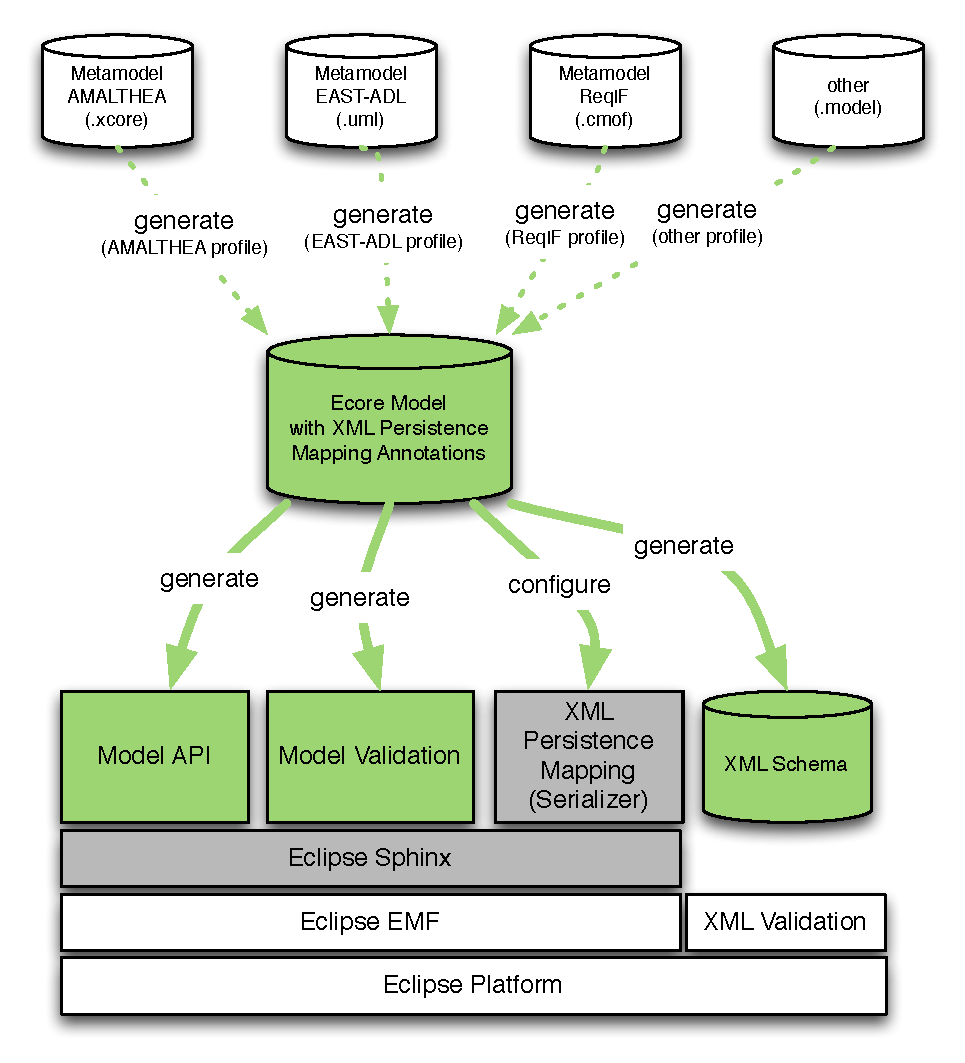
\includegraphics[width=\textwidth]{images/XMLPersistenceMapping_Overview.pdf}
\caption{From Domain Model to Tool and XSD}
\label{fig:XMLPersistenceMapping_Overview}
\end{figure}

\begin{figure}[hpt]
\centering
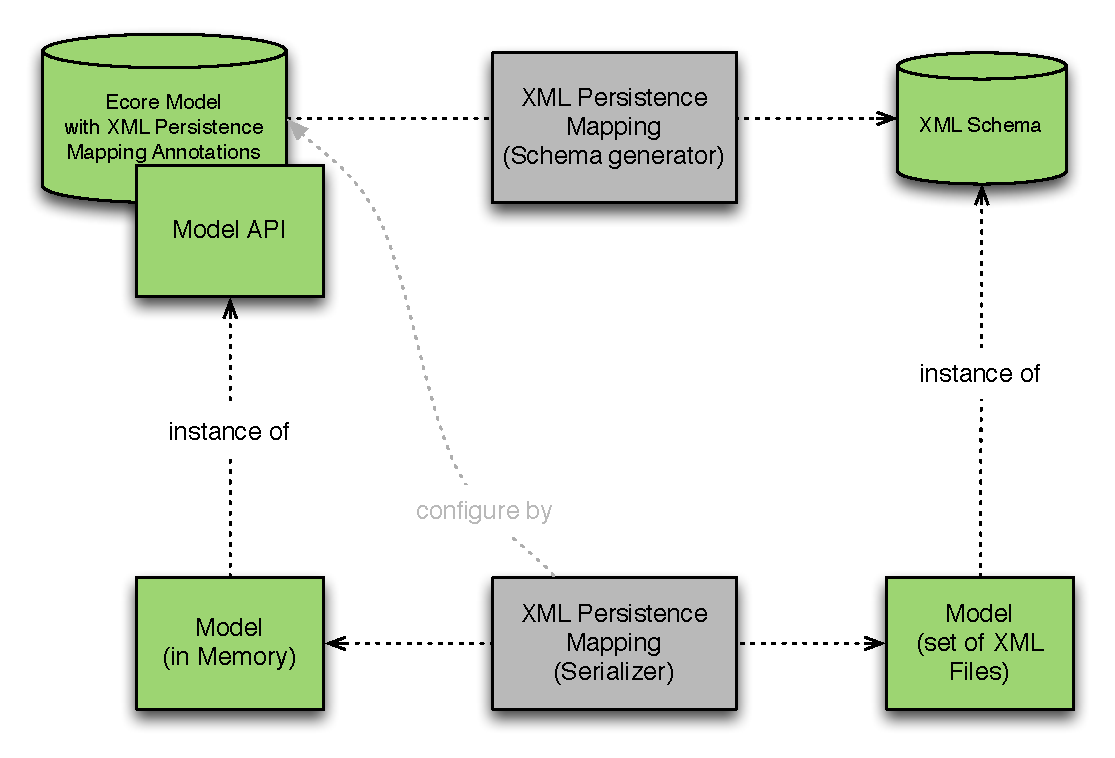
\includegraphics[width=\textwidth]{images/XMLPersistenceMapping_SerializerAndGenerator.pdf}
\caption{XML Persistence Mapping: Relation between XSD Schema generator and Serializer}
\label{fig:XMLPersistenceMapping_SerializerAndGenerator}
\end{figure}

\addtodo{add motivation: interoperability}\\
\addtodo{add motivation: performance, memory consumption}\\

\section{Use Cases}
\addtodo{overview}\\

\subsection{Variant Handling}
\addtodo{Formulate the use cases as agile user stories}\\
The XML persistence mapping shall support variant handling on file level. E.g. it shall be possible to store the overall model in several files and to select a variant by exchanging individual XML files.

\subsection{Machine Readability}
\addtodo{complex systems as well as simple scripts}\\


\subsection{Human Readability}
As an engineer I want to be able to create, read, update and delete XML files according to the XML persistence mapping rules so that I can validate and customize the overall model manually a generic XML editor in case no high-level tools are available yet. \\
Pattern that support human readability are:
\begin{itemize}
\item wrapper XML elements that support folding and unfolding of lists
\item consistent naming conventions for mapping between the model and the XML-representation
\item strict rules for usage of XML elements and XML attributes
\item syntax completion by providing an XML schema to the XML editor 
\end{itemize}

\subsection{Validation}
As an end-user I want to validate individual XML files against an XML Schema so that I can execute an initial quality check by means of generic XML Schema validators.

\subsection{Text Diff}
As an end-user I want to apply a textual diff tool on different versions of the XML files so that I can identify the model differences on file level.
This requires deterministic and one-to-one persistence mapping between the model in memory and its XML representation. \\
\addtodo{move solution to section design principles}
Patterns are:
\begin{itemize}
\item defined sequence of XML elements
\item defined sequence of XML attributes
\item preserve order of items in collections
\end{itemize}

\subsection{Full support of existing EMF persistence}
As a tool developer I want to laverage all existing serialization features that are provided by the Eclipse EMF project so that I can still read and write models that do not explicitly support the XML persistence mapping extensions.

\subsection{Model Evolution / Backwards compatibility}

\subsection{Manual annotation of metamodel}
As a developer I want to efficiently be able to directly create and annotate my XCore or Ecore model as an input for the XML persistence mapping. E.g. I want to configure the default persistence mapping strategies at a central location so I do not need to add annotations to all model elements which might reduce the readability of my model.

\section{Related Standards and Specifications}
The following figure illustrates the relation and dependencies between the related standards:
\begin{figure}
\centering
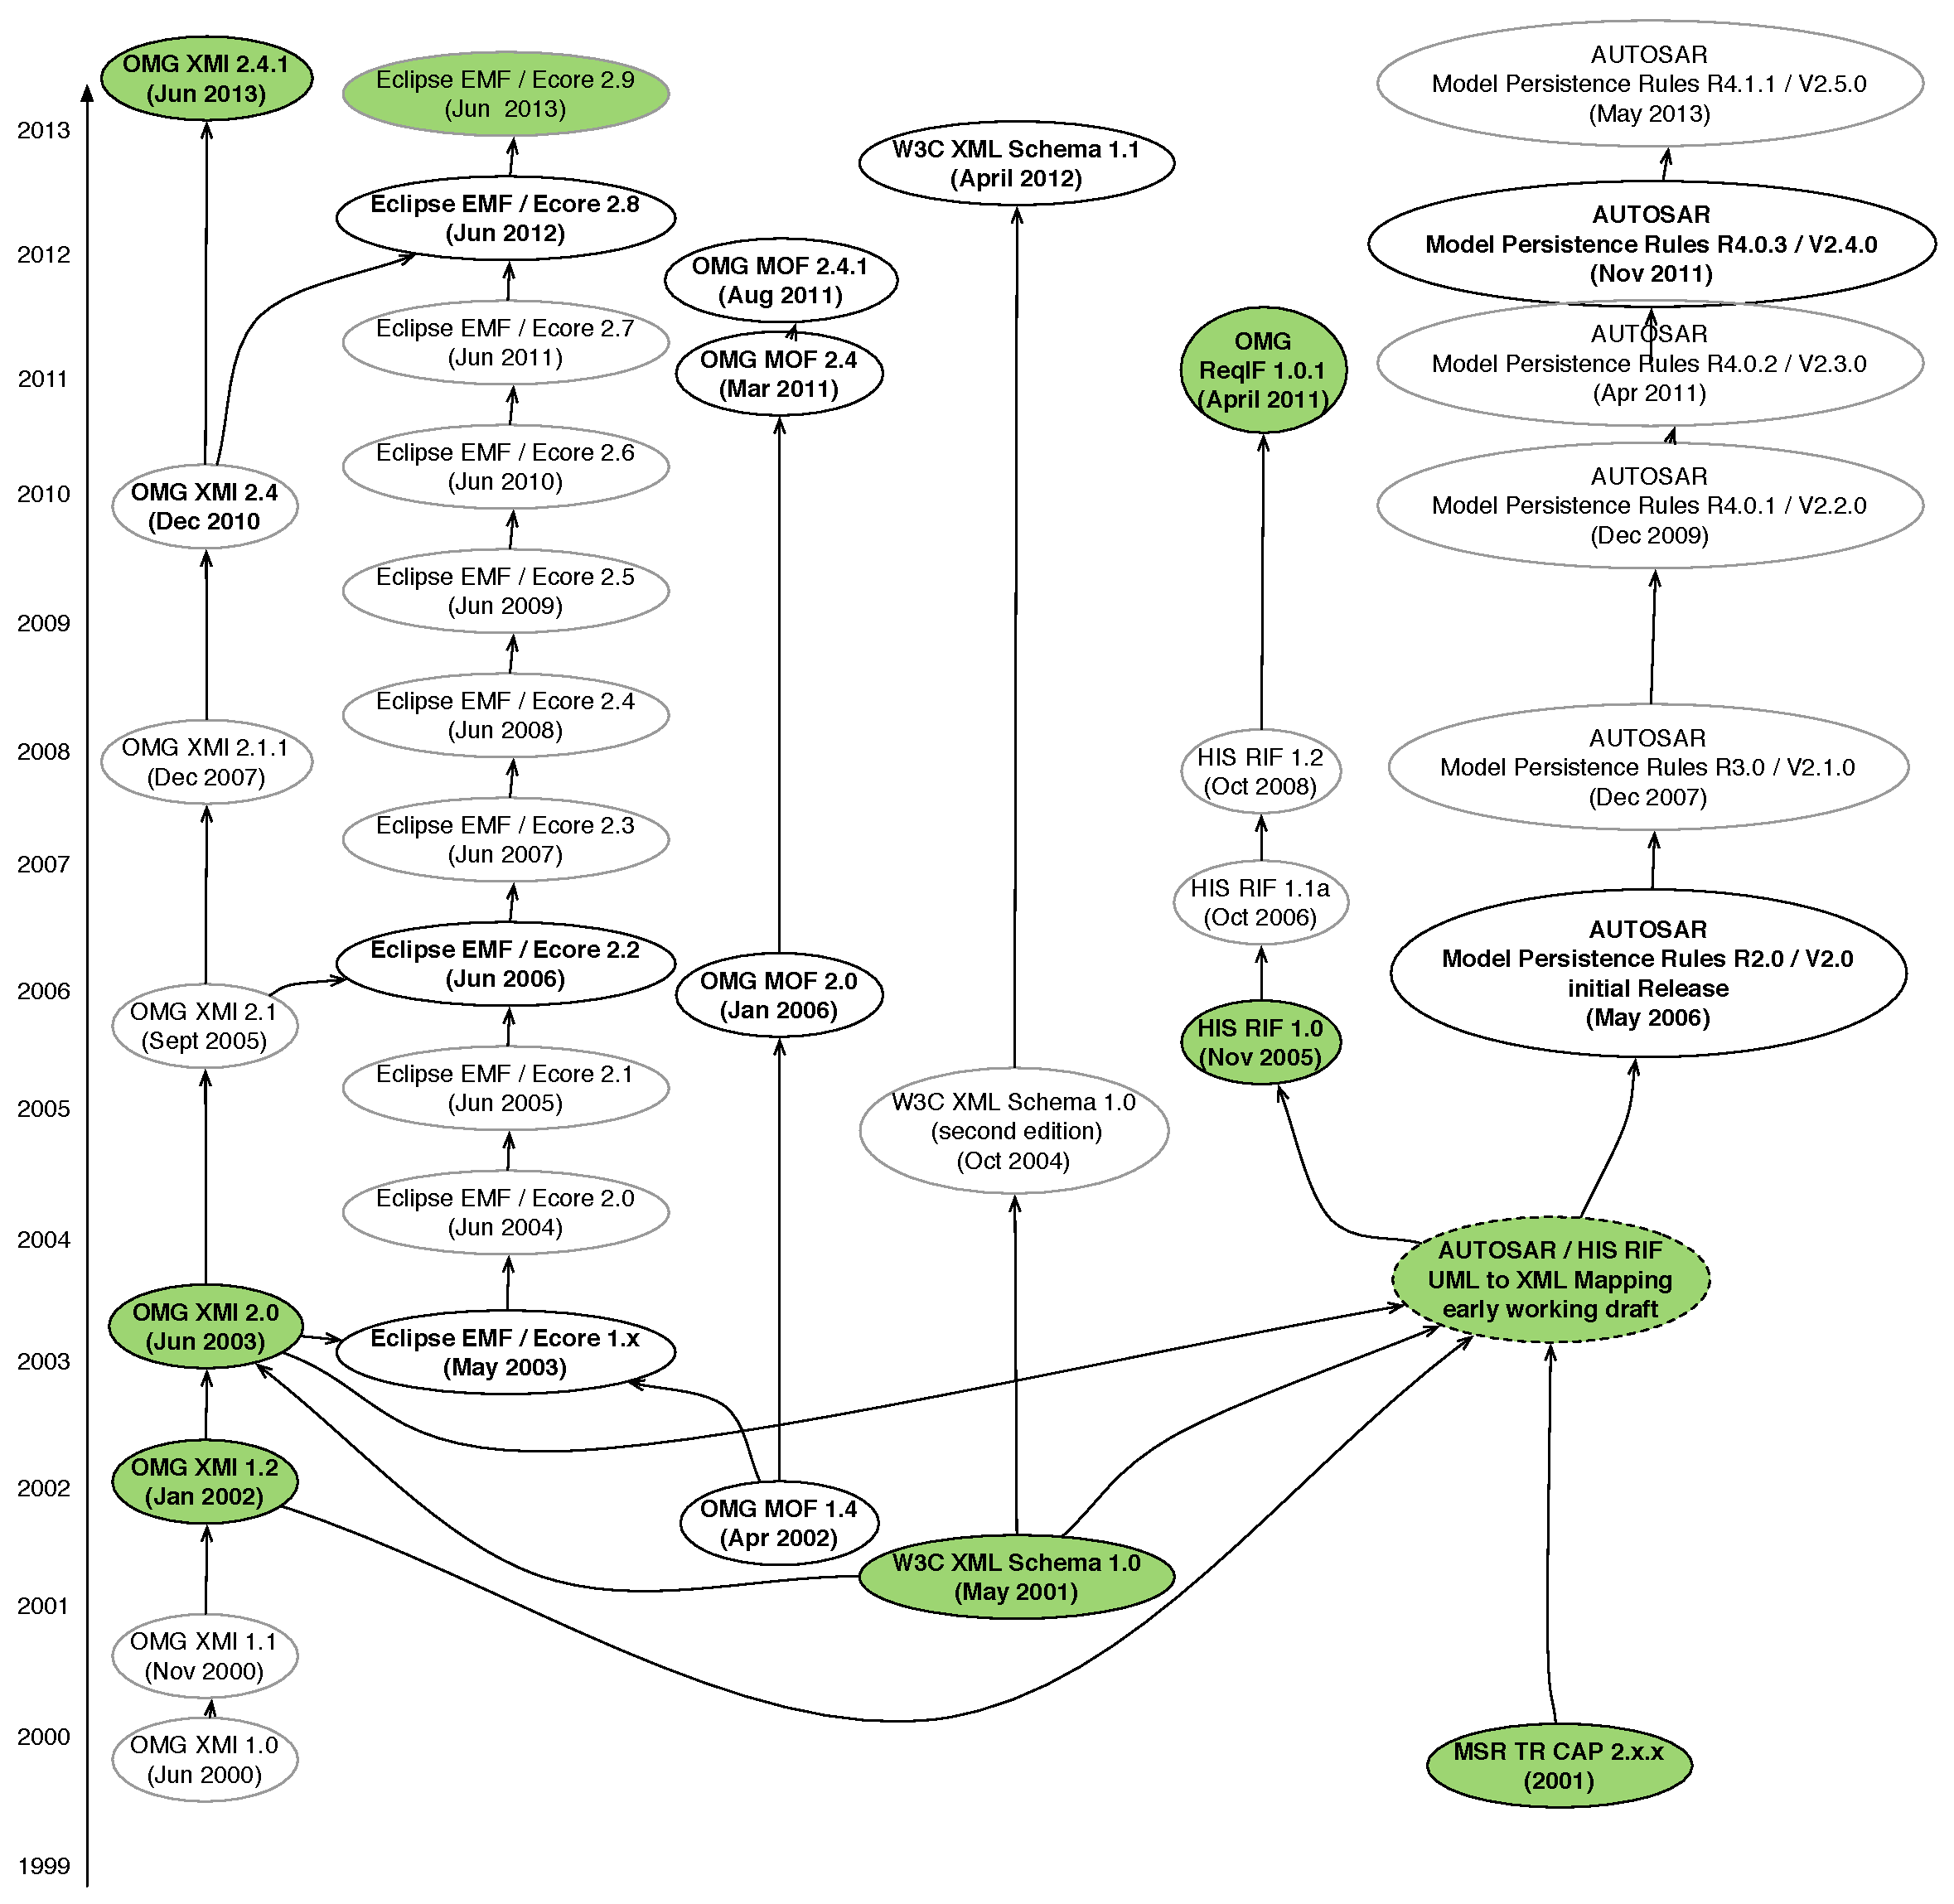
\includegraphics[width=\textwidth]{images/XMLPersistenceMapping_RelatedStandards.pdf}
\end{figure}

\subsection{OMG XMI}
The OMG MOF 2 XMI Mapping specifications describe how to exchange metadata and models by means of XML files. The 2.x versions of the XMI standard are fundamentally different from the 1.x versions:
\begin{itemize}
\item XMI 1.x describes mapping rules between MOF and XML DTDs. Example of an UML model serialized using XMI 1.2 \cite{omg:xmi12}:
\inputminted[fontsize=\footnotesize, tabsize=2]{xml}{examples/XMI12_Example.xml}

\item XMI 2.x describes mapping rules between MOF and XML Schema. These mappings produce more compact XML files. Example of an UML model serialized using XMI 2.4.1 \cite{omg:xmi241}:
\inputminted[fontsize=\footnotesize, tabsize=2]{xml}{examples/XMI241_Example.xml}
\end{itemize} 

\subsection{OMG ReqIF}

\subsection{EMF XML Mapping}
EMF has implemented XMI 2.x for serialization of models to XMI. Additionally, a more flexible mapping to XML schema is supported \cite{eclipse:xmlschemamapping}.
\addtodo{describe some configuration possibilities and advantages, e.g. feature maps}

\section{Metamodel Best Practices}
\subsection{Ecore Patterns}
\subsubsection{Use primitive types when possible}
Ecore provides several predefined data types. Whenever possible, the datatype that maps to a primitive Java type should be used. 
E.g. a boolean values can be represented by EBoolean (java.lang.boolean) or EBooleanObject (java.lang.Boolean). java.lang.Boolean wraps the primitive type java.lang.boolean and thus adds some overhead with respect to resource consumption. Additionally, wrapping the primitive type into an object adds the additional value 'null' which needs to be handled in your application.

\subsubsection{Explicitly mark features unsetable}
By explicitly setting EStructuralFeatures to unsetable, the EMF Code generator adds flags and and an API that allows tracking if the EStructuralFeature is set.
If the unsetable option is not set, EMF derives that information from the value of the feature: If the value equals to its default value or if a list is empty then it is considered as unset. 
Thus, it is not possible to distinguish between a value that was explicitly set to the default value and a value that was not set at all.\\
\addtodo{add note on additonal memory consumption and how to overcome it}

\subsubsection{Explicitly mark features ordered}
EStructuralFeatures that represent multiple values (isMany()$==$true) can have the semantics of an ordered list or an unordered collection. The semantics of the ordered list should be preferred for the following reasons:
\begin{itemize}
\item preserve the order of elements when reading and writing models (important for textual diff of XML files)
\item deterministic navigation in model is prerequisit for deterministic code generation
\end{itemize}

Note: The EMF code generator currently ignores the 'ordered' property and always generates ELists. However, this might change in future and frameworks such as QVTO or OCL already evaluate the flag.

\subsubsection{Avoid sub packages}
Unless the class names in the model are not unique, nested packages are unnecessary syntactic sugar and often end up causing 
problems because some aspect of the framework doesn't work perfectly for them.


\subsection{EMF Code Generator}

\subsection{Java Performance Tuning}
Performance tuning in Java is highly related to the implementation of the Java Virtual Machine. Please see \cite{merks:performance} for more details.
Additional performance optimizations are described in \cite{steinberg:emfperformance}.\cite{merks:performance} 

\section{XML Best Practices}
\subsection{XML Schema Patterns}
\subsubsection{Use Schema for Validation only}
XML Schema can be used for validation of XML documents as well as a provider of default values. If default values are defined in the XML Schema the XML processor might produce different values if the document is pared with or without availability of the XML Schema. Thus, the XML schema should be used for validation only and no default values should be defined.
\subsubsection{Prefer xsd:sequence}
XML complex types can group the contained XML elements in sequential (xsd:sequence),  disjunctive (xsd:choice) or conjunctive (xsd:all) manner. Whenever applicable, the xsd:sequence pattern schould be preferred since it enforces a given sequence of XML elements in the XML document which simplifies textual diff of XML files.
\subsubsection{Avoid extension or restriction of xsd:complexTypes}
\addtodo{provide more background information: only single inheritance, requires repitition of elements, complex to validate. discuss named xsd:group vs. repitition of elements in each complex type}


\subsection{XML Document Patterns}


\section{Ecore to XML Mapping Design Principles}
\addtodo{principles}\\

\subsection{Overview}

\begin{figure}
\centering
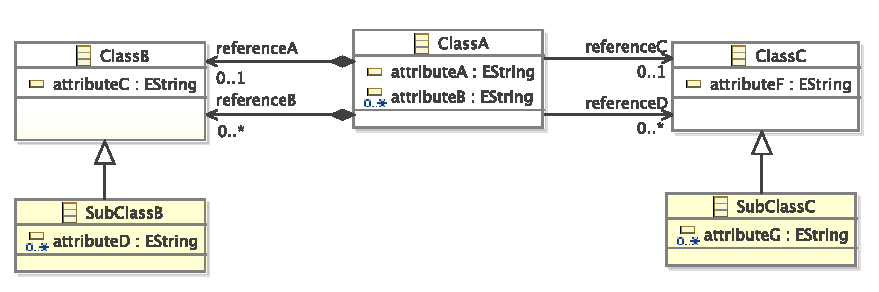
\includegraphics[width=\textwidth]{examples/Design_Principles_Inheritance.pdf}
\end{figure}

\addtodo{what do we need for serialization without loss of information}\\


\subsection{Customization for Different Meta Models}
\addtodo{todo
dependent on primary usecases\\
two step approach\\
Language specific profiles (mapping of annotated UML to fully annotated XML Persistence Mapping Model)\\
Rules described in this document \\}

\subsection{XML Elements vs. Attributes}
\addtodo{XML Elements vs. Attributes}\\

\subsection{XML Version}
\addtodo{Impact Table: Metamodel / Model / XML Schema / Schema}\\


\subsection{Linking}
\addtodo{Linking}\\

\subsection{Null and Default Values}
\addtodo{Null and Default Values}\\

\subsection{Primitive Types}
\addtodo{primitive types: xsd:types vs. refined xsd:strings}\\


\subsection{Packages and Namespaces}
\addtodo{Packages and Namespaces}\\

\subsection{EAttributes with occurance bigger than 1}
Each XML attribute may occur only once in the context of an XML. For mapping of EAttribute that represent a list of values, two alternatives are possible:
\begin{enumerate}
\item Representation by a single XML attribute or XML element which carries the list of values separated by a special character.
\item Representation by multiple XML elements. Each wraps an individual value.
\end{enumerate}

\subsection{Extensions}
\addtodo{AUTOSAR: splittable \\
other concepts}\\


\subsection{Inheritance}
\addtodo{xmi:type vs. xsi:type vs. schema inheritance and restriction}\\


\subsection{Validation}
\addtodo{levels of validation}\\



\section{XML Document Production}
This Chapter contains detailed information for implementers of tools that read and write XML documents according to the XML Persistence Mappings.

\paragraph{EBNF - Syntax Diagram}
\begin{rail}
document : XMLDecl RootObjDecl;
XMLDecl : '<?xml' VersionInfo EncodingDecl? '?>';
VersionInfo : S  'version="' ('1.0'|'1.1') '"';
EncodingDecl : S 'encoding="' Encoding '"';
RootObjDecl : '<' ClassifierName NameSpaceDecl Attributes?'>' \\ 
Elements \\
'</' ClassifierName '>';

Elements : (DocumentEAttributeContained | DocumentEReferenceContained | DocumentEReferenceReferenced)*;
\end{rail}

\begin{rail}
QFeatureWrapperName : ((featureNsPrefix ':')?) featureWrapperName;
QFeatureName : ((featureNsPrefix ':')?) featureName;
ExtClassifierWrapperName : classifierWrapperName classifierWrapperNameSuffix;
ExtClassifierName : classifierName classifierNameSuffix;
QClassifierWrapperName : ((classifierNsPrefix ':')?) classifierWrapperName;
QClasifierName : ((classifierNsPrefix ':')?) classifierName;
QExtClassifierWrapperName : ((classifierNsPrefix ':')?) classifierWrapperName classifierWrapperNameSuffix;
QExtClasifierName : ((classifierNsPrefix ':')?) classifierName classifierNameSuffix;
TypeAttribute : typeAttributeName '=' '"' QExtClassifierName '"';

\end{rail}

%%%%%%%%%%%%%%%%%%%%%%%%%%%%%%%%%%%%%%%%
\subsection{Document Mapping for EAttributeAttribute}

\paragraph{EBNF - Syntax Diagram}

\paragraph{Document Example}

%%%%%%%%%%%%%%%%%%%%%%%%%%%%%%%%%%%%%%%%
\subsection{Document Mappings for EAttributeContained}
This rule maps the EAttribute to an XML element.



\paragraph{Preconditions} 
EAttributeContainedxxxx mappings are applicable if
\begin{align*}
\wedge & \, x \, instanceof \, \text{EAttribute}  \\
\wedge & \, false == x.isTransient()  \\
\wedge & \,  ExtendedMetaData.ELEMENT\_FEATURE == extendedMetaData.getFeatureKind(x) \\
\end{align*}

\paragraph{EBNF - Syntax Diagram}
\begin{rail}
DocumentEAttributeContained : [1]([ ]DocumentEAttributeContained0000 | [ ]DocumentEAttributeContained0001 | [ ]DocumentEAttributeContained0010 | [ ]DocumentEAttributeContained0011 | [2,3]DocumentEAttributeContained0100 | [ ]DocumentEAttributeContained0101 | [ ]DocumentEAttributeContained0110 | [ ]DocumentEAttributeContained0111 | [ ]DocumentEAttributeContained1000 | [ ]DocumentEAttributeContained1001 | [ ]DocumentEAttributeContained1010 | [ ]DocumentEAttributeContained1011 | [3]DocumentEAttributeContained1100 | [ ]DocumentEAttributeContained1101 | [ ]DocumentEAttributeContained1110 | [ ]DocumentEAttributeContained1111);
\end{rail}

\paragraph{Constraints and Parameterization}
\begin{enumerate}
\item Selection of DocumentEAttributeContainedxxxx Rules: \\
\begin{tabular}{l|c|c|c|c|}
\cline{2-5} 
& \multicolumn{4}{ |c| }{XMLPersistenceExtendeMetaData}  \\
\hline
 \multicolumn{1}{ |c| }{Mapping Rule}& feature & feature & classifier  & classifier \\
 \multicolumn{1}{ |c| }{...EAttribute...} & WrapperElement & Element & WrapperElement & Element\\
\hline 
 \multicolumn{1}{ |c| }{not applicable} & false & false & false & false \\
 \multicolumn{1}{ |c| }{...Contained0001} & false & false & false & true \\ 
 \multicolumn{1}{ |c| }{...Contained0010} & false & false & true & false \\
 \multicolumn{1}{ |c| }{...Contained0011} & false & false & true & true \\ 
 \multicolumn{1}{ |c| }{...Contained0100} & false & true & false & false \\ 
 \multicolumn{1}{ |c| }{...Contained0101} & false & true & false & true \\ 
 \multicolumn{1}{ |c| }{...Contained0110} & false & true & true & false \\ 
 \multicolumn{1}{ |c| }{...Contained0111} & false & true & true & true \\ 
 \multicolumn{1}{ |c| }{...Contained1000} & true & false & false & false \\ 
 \multicolumn{1}{ |c| }{...Contained1001} & true & false & false & true \\ 
 \multicolumn{1}{ |c| }{...Contained1010} & true & false & true & false \\ 
 \multicolumn{1}{ |c| }{...Contained1011} & true & false & true & true \\ 
 \multicolumn{1}{ |c| }{...Contained1100} & true & true & false & false \\ 
 \multicolumn{1}{ |c| }{...Contained1101} & true & true & false & true \\
 \multicolumn{1}{ |c| }{...Contained1110} & true & true & true & false \\ 
 \multicolumn{1}{ |c| }{...Contained1111} & true & true & true & true \\ 
\hline
\end{tabular}

\item If XMLPersistenceExtendedMetaData is not defined, then rule DocumentEAttributeContained0100 applies (default EMF persistence behaviour).

\item If XMLPersistenceExtendedMetaData is defined and one of the keys featureWrapperElement, featureElement, classifierWrapperElement, classifierWrapper is missing, then the rule DocumentEAttributeContained1100 applies for EAttributes with $true==x.isMany()$ and rule DocumentEAttributeContained0100 otherwise. Since these missing keys identify an error in the configuration, the (de)serializer shall log an error message.
\end{enumerate}

\paragraph{Description of Example}
The EAttributeContained examples are based on the following minimal ecore model:

\begin{figure}[h]
\centering
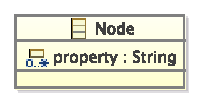
\includegraphics[]{examples/EAttributeContained.pdf}
\end{figure}

\inputminted[firstline=15, fontsize=\footnotesize]{java}{examples/EAttributeContained.xcore}

The model consists of a single 'Node' Object that has two values for the EAttribute 'property': 'Property1' and 'Property2'

\subsubsection{Document Mapping for EAttributeContained0000}
Invalid invalid mapping rule.

\subsubsection{Document Mapping for EAttributeContained0001}
\paragraph{Preconditions}
\addtodo{todo}

\paragraph{EBNF - Syntax Diagram}
\begin{rail}
DocumentEAttributeContained0001 : ((([1]'<' QExtClassifierName' >' \\
value \\
'</' QExtClassifierName '>')+) 
| [2,3]'<' QExtClassifierName S 'xsi:nil' '/>'); 
\end{rail}

\paragraph{Constraints and Parameterization}
\begin{enumerate}
\item If $\neg (obj.eGet(x).isEmpty() \vee null=obj.eGet(x))$ then create start and end XML elements that contain the value
\item If $true = x.isMany() \wedge obj.eGet(x).isEmpty()$ then xsi:nil shall be used.
\item If $false = x.isMany() \wedge true=obj.eIsSet(x) \wedge null=obj.eGet()$ then xsi:nil shall be used.
\end{enumerate}

\addtodo{do we need to handle null values in lists?}: 

\paragraph{Document Example}
\inputminted[fontsize=\footnotesize]{xml}{examples/EAttributeContained0001.xml}

\subsubsection{Document Mapping for EAttributeContained0010}
\paragraph{EBNF - Syntax Diagram}
\begin{rail}
DocumentEAttributeContained0010 :
[1]((([2]'<' QExtClassifierWrapperName '>'\\
([3]value ((' ' value)*)) \\
'</' QExtClassifierWrapperName '>'))
| '<' QExtClassifierWrapperName S 'xsi:nil' '/>')
\end{rail}

\paragraph{Document Example}
\inputminted[fontsize=\footnotesize]{xml}{examples/EAttributeContained0010.xml}

\subsubsection{Document Mapping for EAttributeContained0011}
\paragraph{EBNF - Syntax Diagram}
\begin{rail}
DocumentEAttributeContained0011 :
([1]('<' QExtClassifierWrapperName' >'\\
([2]([3]'<' QExtClassifierName '>' \\
value \\
'</' QExtClassifierName '>')*) \\
'</' QExtClassifierWrapperName' >'))
\end{rail}

\paragraph{Document Example}
\inputminted[fontsize=\footnotesize]{xml}{examples/EAttributeContained0011.xml}


\subsubsection{Document Mapping for EAttributeContained0100}
\paragraph{EBNF - Syntax Diagram}
\begin{rail}
DocumentEAttributeContained0100 : [1]((([2]'<' QFeatureName '>' \\
value \\ 
'</' QFeatureName' >')+) 
| '<' QFeatureName S 'xsi:nil' '/>'); 
\end{rail}

\paragraph{Document Example}
\inputminted[fontsize=\footnotesize]{xml}{examples/EAttributeContained0100.xml}

\subsubsection{Document Mapping for EAttributeContained0101}
\paragraph{EBNF - Syntax Diagram}
\begin{rail}
DocumentEAttributeContained0101 : [1]('<' QFeatureName '>' ([2]('<' QExtClassifierName '>' \\
value \\
'</' QExtClassifierName '>')?)\\
'</' QFeatureName' >')+; 
\end{rail}

\paragraph{Document Example}
\inputminted[fontsize=\footnotesize]{xml}{examples/EAttributeContained0101.xml}

\subsubsection{Document Mapping for EAttributeContained0110}
\paragraph{EBNF - Syntax Diagram}
\begin{rail}
DocumentEAttributeContained0110 : [1]('<' QFeatureName '>'  ([2]([3]'<' QExtClassifierWrapperName '>'\\
([4]value ((' ' value)*)) \\
'</' QExtClassifierWrapperName '>')?) \\
'</' QFeatureName '>'); 
\end{rail}

\paragraph{Document Example}
\inputminted[fontsize=\footnotesize]{xml}{examples/EAttributeContained0110.xml}

\subsubsection{Document Mapping for EAttributeContained0111}
\paragraph{EBNF - Syntax Diagram}
\begin{rail}
DocumentEAttributeContained0111 : [1]'<' QFeatureName '>'  \\
([2]([3]'<' QExtClassifierWrapperName '>'\\
(([4]'<' QExtClassifierName' >' \\
value \\
'</' QExtClassifierName '>')+) \\
'</' QExtClassifierWrapperName '>')?)\\
'</' QFeatureName '>'; 
\end{rail}

\paragraph{Document Example}
\inputminted[fontsize=\footnotesize]{xml}{examples/EAttributeContained0111.xml}

\subsubsection{Document Mapping for EAttributeContained1000}
\paragraph{EBNF - Syntax Diagram}
\begin{rail}
DocumentEAttributeContained1000 : [1](('<' QFeatureWrapperName '>' \\
([2]value ((' ' value)*)) \\
'</' QFeatureWrapperName '>')
 | '<' QFeatureWrapperName S 'xsi:nil' '/>');
\end{rail}

\paragraph{Document Example}
\inputminted[fontsize=\footnotesize]{xml}{examples/EAttributeContained1000.xml}


\subsubsection{Document Mapping for EAttributeContained1001}
\paragraph{EBNF - Syntax Diagram}
\begin{rail}
DocumentEAttributeContained1001 : [1]'<' QFeatureWrapperName '>' \\
([2]([3]'<' QExtClassifierName '>' value '</' QExtClassifierName '>')*) \\
'</' QFeatureWrapperName '>' ;
\end{rail}

\paragraph{Document Example}
\inputminted[fontsize=\footnotesize]{xml}{examples/EAttributeContained1001.xml}


\subsubsection{Document Mapping for EAttributeContained1010}
\paragraph{EBNF - Syntax Diagram}
\begin{rail}
DocumentEAttributeContained1010 : [1]'<' QFeatureWrapperName '>' \\
([2]([3]'<' QExtClassifierWrapperName '>' \\
([4]value ((' ' value)*)) \\
'</' QExtClassifierWrapperName '>') ?) \\
'</' QFeatureWrapperName '>' ;
\end{rail}

\paragraph{Document Example}
\inputminted[fontsize=\footnotesize]{xml}{examples/EAttributeContained1010.xml}

\subsubsection{Document Mapping for EAttributeContained1011}
\paragraph{EBNF - Syntax Diagram}
\begin{rail}
DocumentEAttributeContained1011 : [1]'<' QFeatureWrapperName '>' \\
([2]([3]'<' QExtClassifierWrapperName '>' \\
([4]('<' QExtClassifierName '>' \\
value \\
'</' QExtClassifierName '>')+) \\
'</' QExtClassifierWrapperName '>')?)\\
'</' QFeatureWrapperName '>' ;
\end{rail}
\paragraph{Document Example}
\inputminted[fontsize=\footnotesize]{xml}{examples/EAttributeContained1011.xml}

%%%%%%%%%%%%%%%%%%%
\subsubsection{Document Mapping for EAttributeContained1100}
\paragraph{EBNF - Syntax Diagram}
\begin{rail}
DocumentEAttributeContained1100 : [1]'<' QFeatureWrapperName '>' \\
([2]([3]'<' QFeatureName '>'  \\
value \\
'</' QFeatureName '>')*) \\
'</' QFeatureWrapperName '>' ;
\end{rail}

\paragraph{Document Example}
\inputminted[fontsize=\footnotesize]{xml}{examples/EAttributeContained1100.xml}

%%%%%%%%%%%%%%%%%%%
\subsubsection{Document Mapping for EAttributeContained1101}
\paragraph{EBNF - Syntax Diagram}
\begin{rail}
DocumentEAttributeContained1101 : [1]'<' QFeatureWrapperName '>' \\
([2]([3]'<' QFeatureName '>' \\
([4]('<' QExtClassifierName '>' \\
value\\
'</' QExtClassifierName '>')) \\
'</' QFeatureName '>')*) \\
'</' QFeatureWrapperName '>' ;
\end{rail}
\paragraph{Document Example}
\inputminted[fontsize=\footnotesize]{xml}{examples/EAttributeContained1101.xml}


\subsubsection{Document Mapping for EAttributeContained1110}
\paragraph{EBNF - Syntax Diagram}
\begin{rail}
DocumentEAttributeContained1110 : [1]'<' QFeatureWrapperName '>' \\
([2]([3]'<' QFeatureName '>' '<' QExtClassifierWrapperName '>' \\
([4]value ((' ' value)*)) \\
'</' QExtClassifierWrapperName '>' '</' QFeatureName '>')?) \\
'</' QFeatureWrapperName '>' ;
\end{rail}

\paragraph{Document Example}
\inputminted[fontsize=\footnotesize]{xml}{examples/EAttributeContained1110.xml}


\subsubsection{Document Mapping for EAttributeContained1111}
\paragraph{EBNF - Syntax Diagram}
\begin{rail}
DocumentEAttributeContained1111 : '<' QFeatureWrapperName '>' \\
([1]('<' QFeatureName '>'  ('<' QExtClassifierWrapperName '>'\\
([2]('<' QExtClassifierName '>'\\
 value \\
 '</' QExtClassifierName '>')+) \\
'</' QExtClassifierWrapperName '>') '</' QFeatureName '>')?) \\
'</' QFeatureWrapperName '>' ;
\end{rail}
\paragraph{Document Example}
\inputminted[fontsize=\footnotesize]{xml}{examples/EAttributeContained1111.xml}

%%%%%%%%%%%%%%%%%%%%%%%%%%%%%%%%%%%%%
\subsection{Document Mappings for containment EReferences}
\paragraph{Preconditions} 
Document mapping is applicable if
\begin{align*}
& \, false == x.isTransient()  \\
\wedge & \, true == x.isContainment() \\
\wedge & \,  ExtendedMetaData.ELEMENT\_FEATURE == extendedMetaData.getFeatureKind(x) \\
\end{align*}

\paragraph{EBNF - Syntax Diagram}
\begin{rail}
DocumentEReferenceContained : [1](DocumentEReferenceContained0000 | DocumentEReferenceContained0001 | DocumentEReferenceContained0010 | DocumentEReferenceContained0011 | DocumentEReferenceContained0100 | DocumentEReferenceContained0101 | DocumentEReferenceContained0110 | DocumentEReferenceContained0111 | DocumentEReferenceContained1000 | DocumentEReferenceContained1001 | DocumentEReferenceContained1010 | DocumentEReferenceContained1011 | DocumentEReferenceContained1100 | DocumentEReferenceContained1101 | DocumentEReferenceContained1110 | DocumentEReferenceContained1111);
\end{rail}

\paragraph{Note 1}
\begin{center}
\begin{tabular}{l|c|c|c|c|}
\cline{2-5} 
& \multicolumn{4}{ |c| }{XMLPersistenceExtendeMetaData}  \\
\hline
  \multicolumn{1}{ |c| }{}& feature & feature & classifier  & classifier \\
 \multicolumn{1}{ |c| }{Mapping Rule} & WrapperElement & Element & WrapperElement & Element\\
\hline 
 \multicolumn{1}{ |c| }{...EReferenceContained0000} & false & false & false & false \\
 \multicolumn{1}{ |c| }{...EReferenceContained0001} & false & false & false & true \\ 
 \multicolumn{1}{ |c| }{...EReferenceContained0010} & false & false & true & false \\
 \multicolumn{1}{ |c| }{...EReferenceContained0011} & false & false & true & true \\ 
 \multicolumn{1}{ |c| }{...EReferenceContained0100} & false & true & false & false \\ 
 \multicolumn{1}{ |c| }{...EReferenceContained0101} & false & true & false & true \\ 
 \multicolumn{1}{ |c| }{...EReferenceContained0110} & false & true & true & false \\ 
 \multicolumn{1}{ |c| }{...EReferenceContained0111} & false & true & true & true \\ 
 \multicolumn{1}{ |c| }{...EReferenceContained1000} & true & false & false & false \\ 
 \multicolumn{1}{ |c| }{...EReferenceContained1001} & true & false & false & true \\ 
 \multicolumn{1}{ |c| }{...EReferenceContained1010} & true & false & true & false \\ 
 \multicolumn{1}{ |c| }{...EReferenceContained1011} & true & false & true & true \\ 
 \multicolumn{1}{ |c| }{...EReferenceContained1100} & true & true & false & false \\ 
 \multicolumn{1}{ |c| }{...EReferenceContained1101} & true & true & false & true \\
 \multicolumn{1}{ |c| }{...EReferenceContained1110} & true & true & true & false \\ 
 \multicolumn{1}{ |c| }{...EReferenceContained1111} & true & true & true & true \\ 
\hline
\end{tabular}
\end{center}

The following default mapping rules apply:
\begin{itemize}
\item If XMLPersistenceExtendedMetaData is not defined, then rule DocumentEReferenceContained0100 applies (default EMF persistence behaviour).
\item If XMLPersistenceExtendedMetaData is defined and one of the keys featureWrapperElement, featureElement, classifierWrapperElement, classifierWrapper is missing, then the rule DocumentEReferenceContained1001 applies for EReferences with $true==x.isMany()$ and rule DocumentEReferenceContained0101 otherwise. Since these missing keys identify an error in the configuration, the (de)serializer shall log an error message.
\end{itemize}

\subsubsection{Document Mapping for EReferenceContained0000}
\addtodo{todo}
\paragraph{Document Example}
\inputminted[fontsize=\footnotesize]{xml}{examples/EReferenceContained0000.xml}

\subsubsection{Document Mapping for EReferenceContained0001}
\paragraph{EBNF - Syntax Diagram}
\begin{rail}
DocumentEReferenceContained0001 : [1]((([2]'<' QExtClassifierName    Attributes ' >' \\
Elements \\
'</' QExtClassifierName   '>')+) 
| '<' QExtClassifierName  S 'xsi:nil' '/>'); 
\end{rail}
\paragraph{Document Example}
\inputminted[fontsize=\footnotesize]{xml}{examples/EReferenceContained0001.xml}
%%%%%%%%%%%%%%


\subsubsection{Document Mapping for EReferenceContained0010}
\paragraph{EBNF - Syntax Diagram}
\begin{rail}
DocumentEReferenceContained0010 :
[1](([2]'<' QExtClassifierWrapperName   '>'\\
([3]Elements*) \\
'</' QExtClassifierWrapperName  '>')+)
\end{rail}
\paragraph{Document Example}
\inputminted[fontsize=\footnotesize]{xml}{examples/EReferenceContained0010.xml}
%%%%%%%%%%%%%%

\subsubsection{Document Mapping for EReferenceContained0011}
\paragraph{EBNF - Syntax Diagram}
\begin{rail}
DocumentEReferenceContained0011 :
([1]('<' QExtClassifierWrapperName  ' >'\\
([2]([3]'<' QExtClassifierName  Attributes '>' \\
Elements \\
'</' QExtClassifierName  '>')*) \\
'</' QExtClassifierWrapperName   '>')+)
\end{rail}
\paragraph{Document Example}
\inputminted[fontsize=\footnotesize]{xml}{examples/EReferenceContained0011.xml}
%%%%%%%%%%%%%%

\subsubsection{Document Mapping for EReferenceContained0100}
\paragraph{EBNF - Syntax Diagram}
\begin{rail}
DocumentEReferenceContained0100 : [1]((([2]'<' QFeatureName Attributes \\
TypeAttribute? '>' \\
Elements \\ 
'</' QFeatureName' >')+) 
| '<' QFeatureName S 'xsi:nil' '/>'); 
\end{rail}
\paragraph{Document Example}
\inputminted[fontsize=\footnotesize]{xml}{examples/EReferenceContained0100.xml}
%%%%%%%%%%%%%%

\subsubsection{Document Mapping for EReferenceContained0101}
\paragraph{EBNF - Syntax Diagram}
\begin{rail}
DocumentEReferencedContained0101 : [1]('<' QFeatureName '>' \\
([2]('<' QExtClassifierName  Attributes '>' \\
Elements \\
'</' QExtClassifierName  '>')?)\\
'</' QFeatureName' >')+; 
\end{rail}
\paragraph{Document Example}
\inputminted[fontsize=\footnotesize]{xml}{examples/EReferenceContained0101.xml}
%%%%%%%%%%%%%%

\subsubsection{Document Mapping for EReferenceContained0110}
\paragraph{EBNF - Syntax Diagram}
\begin{rail}
DocumentEReferenceContained0110 : [1]('<' QFeatureName '>'  \\
([2]([3]'<' QExtClassifierWrapperName  '>'\\
([4]Elements+) \\
'</' QExtClassifierWrapperName  '>')*) \\
'</' QFeatureName '>'); 
\end{rail}
\paragraph{Document Example}
\inputminted[fontsize=\footnotesize]{xml}{examples/EReferenceContained0110.xml}
%%%%%%%%%%%%%%

\subsubsection{Document Mapping for EReferenceContained0111}
\paragraph{EBNF - Syntax Diagram}
\begin{rail}
DocumentEReferenceContained0111 : [1]'<' QFeatureName '>'  \\
([2]([3]'<' QExtClassifierWrapperName  '>'\\
(([4]'<' QExtClassifierName   Attributes ' >' \\
Elements \\
'</' QExtClassifierName   '>')+) \\
'</' QExtClassifierWrapperName   '>')*)\\
'</' QFeatureName '>'; 
\end{rail}
\paragraph{Document Example}
\inputminted[fontsize=\footnotesize]{xml}{examples/EReferenceContained0111.xml}
%%%%%%%%%%%%%%

\subsubsection{Document Mapping for EReferenceContained1000}
\paragraph{EBNF - Syntax Diagram}
\begin{rail}
DocumentEReferenceContained1000 : [1]('<' QFeatureWrapperName '>' \\
([2]Elements*) \\
'</' QFeatureWrapperName '>');
\end{rail}
\paragraph{Document Example}
\inputminted[fontsize=\footnotesize]{xml}{examples/EReferenceContained1000.xml}
%%%%%%%%%%%%%%

\subsubsection{Document Mapping for EReferenceContained1001}
\paragraph{EBNF - Syntax Diagram}
\begin{rail}
DocumentEReferenceContained1001 : [1]'<' QFeatureWrapperName '>' \\
([2]([3]'<' QExtClassifierName   Attributes '>' \\
Elements\\
 '</' QExtClassifierName  '>')*) \\
'</' QFeatureWrapperName '>' ;
\end{rail}
\paragraph{Document Example}
\inputminted[fontsize=\footnotesize]{xml}{examples/EReferenceContained1001.xml}
%%%%%%%%%%%%%%

\subsubsection{Document Mapping for EReferenceContained1010}
\paragraph{EBNF - Syntax Diagram}
\begin{rail}
DocumentEReferenceContained1010 : [1]'<' QFeatureWrapperName '>' \\
([2]([3]'<' QExtClassifierWrapperName  '>' \\
([4]Elements+) \\
'</' QExtClassifierWrapperName  '>') *) \\
'</' QFeatureWrapperName '>' ;
\end{rail}
\paragraph{Document Example}
\inputminted[fontsize=\footnotesize]{xml}{examples/EReferenceContained1010.xml}
%%%%%%%%%%%%%%

\subsubsection{Document Mapping for EReferenceContained1011}
\paragraph{EBNF - Syntax Diagram}
\begin{rail}
DocumentEReferenceContained1011 : [1]'<' QFeatureWrapperName '>' \\
([2]([3]'<' QExtClassifierWrapperName  '>' \\
([4]('<' QExtClassifierName  Attributes '>' \\
Elements \\
'</' QExtClassifierName  '>')+) \\
'</' QExtClassifierWrapperName  '>')*)\\
'</' QFeatureWrapperName '>' ;
\end{rail}
\paragraph{Document Example}
\inputminted[fontsize=\footnotesize]{xml}{examples/EReferenceContained1011.xml}
%%%%%%%%%%%%%%

\subsubsection{Document Mapping for EReferenceContained1100}
\paragraph{EBNF - Syntax Diagram}
\begin{rail}
DocumentEReferenceContained1100 : [1]'<' QFeatureWrapperName '>' \\
([2]([3]'<' QFeatureName Attributes \\
TypeAttribute? '>'  \\
Elements \\
'</' QFeatureName '>')*) \\
'</' QFeatureWrapperName '>' ;
\end{rail}
\paragraph{Document Example}
\inputminted[fontsize=\footnotesize]{xml}{examples/EReferenceContained1100.xml}
%%%%%%%%%%%%%%

\subsubsection{Document Mapping for EReferenceContained1101}
\paragraph{EBNF - Syntax Diagram}
\begin{rail}
DocumentEReferenceContained1101 : [1]'<' QFeatureWrapperName '>' \\
([2]([3]'<' QFeatureName '>' \\
([4]('<' QExtClassifierName  Attributes '>' \\
Elements \\
'</' QExtClassifierName  '>')) \\
'</' QFeatureName '>')*) \\
'</' QFeatureWrapperName '>' ;
\end{rail}
\paragraph{Document Example}
\inputminted[fontsize=\footnotesize]{xml}{examples/EReferenceContained1101.xml}
%%%%%%%%%%%%%%

\subsubsection{Document Mapping for EReferenceContained1110}
\paragraph{EBNF - Syntax Diagram}
\begin{rail}
DocumentEReferenceContained1110 : [1]'<' QFeatureWrapperName '>' \\
([2]([3]'<' QFeatureName '>' \\
(('<' QExtClassifierWrapperName  '>' \\
([4]Elements+) \\
'</' QExtClassifierWrapperName  '>')+)\\
 '</' QFeatureName '>')?) \\
'</' QFeatureWrapperName '>' ;
\end{rail}
\paragraph{Document Example}
\inputminted[fontsize=\footnotesize]{xml}{examples/EReferenceContained1110.xml}
%%%%%%%%%%%%%%

\subsubsection{Document Mapping for EReferenceContained1111}
\paragraph{EBNF - Syntax Diagram}
\begin{rail}
DocumentEReferenceContained1111 : '<' QFeatureWrapperName '>' \\
([1]('<' QFeatureName '>' \\
(('<' QExtClassifierWrapperName  '>' \\
([2]('<' QExtClassifierName  \\ Attributes '>' \\
Elements \\
'</' QExtClassifierName  '>')+) \\
'</' QExtClassifierWrapperName  '>')+) \\
'</' QFeatureName '>')?) \\
'</' QFeatureWrapperName '>' ;
\end{rail}

\paragraph{Document Example}
\inputminted[fontsize=\footnotesize]{xml}{examples/EReferenceContained1111.xml}
%%%%%%%%%%%%%%

\subsection{Document Mappings for non-containment EReferences}
\paragraph{Preconditions} 
Document mapping is applicable if
\begin{align*}
& \, false == x.isTransient()  \\
\wedge & \,  false == x.isContainment() \\
\wedge & \,  ExtendedMetaData.ELEMENT\_FEATURE == extendedMetaData.getFeatureKind(x) \\
\end{align*}


\begin{rail}
DocumentEReferenceReferenced : (DocumentEReferenceReferenced0000 | DocumentEReferenceReferenced0001 | DocumentEReferenceReferenced0010 | DocumentEReferenceReferenced0011 | DocumentEReferenceReferenced0100 | DocumentEReferenceReferenced0101 | DocumentEReferenceReferenced0110 | DocumentEReferenceReferenced0111 | DocumentEReferenceReferenced1000 | DocumentEReferenceReferenced1001 | DocumentEReferenceReferenced1010 | DocumentEReferenceReferenced1011 | DocumentEReferenceReferenced1100 | DocumentEReferenceReferenced1101 | DocumentEReferenceReferenced1110 | DocumentEReferenceReferenced1111);
\end{rail}

\paragraph{Note 1}
\begin{center}
\begin{tabular}{l|c|c|c|c|}
\cline{2-5} 
& \multicolumn{4}{ |c| }{XMLPersistenceExtendeMetaData}  \\
\hline
  \multicolumn{1}{ |c| }{}& feature & feature & classifier  & classifier \\
 \multicolumn{1}{ |c| }{Mapping Rule} & WrapperElement & Element & WrapperElement & Element\\
\hline 
 \multicolumn{1}{ |c| }{...EReferenceReferenced0000} & false & false & false & false \\
 \multicolumn{1}{ |c| }{...EReferenceReferenced0001} & false & false & false & true \\ 
 \multicolumn{1}{ |c| }{...EReferenceReferenced0010} & false & false & true & false \\
 \multicolumn{1}{ |c| }{...EReferenceReferenced0011} & false & false & true & true \\ 
 \multicolumn{1}{ |c| }{...EReferenceReferenced0100} & false & true & false & false \\ 
 \multicolumn{1}{ |c| }{...EReferenceReferenced0101} & false & true & false & true \\ 
 \multicolumn{1}{ |c| }{...EReferenceReferenced0110} & false & true & true & false \\ 
 \multicolumn{1}{ |c| }{...EReferenceReferenced0111} & false & true & true & true \\ 
 \multicolumn{1}{ |c| }{...EReferenceReferenced1000} & true & false & false & false \\ 
 \multicolumn{1}{ |c| }{...EReferenceReferenced1001} & true & false & false & true \\ 
 \multicolumn{1}{ |c| }{...EReferenceReferenced1010} & true & false & true & false \\ 
 \multicolumn{1}{ |c| }{...EReferenceReferenced1011} & true & false & true & true \\ 
 \multicolumn{1}{ |c| }{...EReferenceReferenced1100} & true & true & false & false \\ 
 \multicolumn{1}{ |c| }{...EReferenceReferenced1101} & true & true & false & true \\
 \multicolumn{1}{ |c| }{...EReferenceReferenced1110} & true & true & true & false \\ 
 \multicolumn{1}{ |c| }{...EReferenceReferenced1111} & true & true & true & true \\ 
\hline
\end{tabular}
\end{center}

The following default mapping rules apply:
\begin{itemize}
\item If XMLPersistenceExtendedMetaData is not defined, then rule DocumentEReferenceReferenced0100 applies (default EMF persistence behaviour).
\item If XMLPersistenceExtendedMetaData is defined and one of the keys featureWrapperElement, featureElement, classifierWrapperElement, classifierWrapper is missing, then the rule DocumentEReferenceReferenced1100 applies for EReferences with $true==x.isMany()$ and rule DocumentEReferenceReferenced0100 otherwise. Since these missing keys identify an error in the configuration, the (de)serializer shall log an error message.
\end{itemize}


\subsubsection{Document Mapping for EReferenceReferenced0000}
not applicable

\subsubsection{Document Mapping for EReferenceReferenced0001}
\paragraph{EBNF - Syntax Diagram}
\begin{rail}
DocumentEReferenceReferenced0001 : (([3]'<' QExtClassifierName  '>' \\ 
targetURI \\ 
'</' QExtClassifierName  '>')+)
\end{rail}

\paragraph{Document Example}
\inputminted[fontsize=\footnotesize]{xml}{examples/EReferenceReferenced0001.xml}


%%%%%%%%%%%%%%%%%%%%%%%%%%%%%%%%%%%%%%%%%%%%
\subsubsection{Document Mapping for EReferenceReferenced0010}
\paragraph{EBNF - Syntax Diagram}
\begin{rail}
DocumentEReferenceReferenced0010 : (([2]'<' QExtClassifierWrapperName '>'\\
(targetURI ((' ' targetURI)*)) \\
'</' QExtClassifierWrapperName '>')+);
\end{rail}

\paragraph{Document Example}
\inputminted[fontsize=\footnotesize]{xml}{examples/EReferenceReferenced0010.xml}


%%%%%%%%%%%%%%%%%%%%%%%%%%%%%%%%%%%%%%%%%%%%
\subsubsection{Document Mapping for EReferenceReferenced0011}
\paragraph{EBNF - Syntax Diagram}
\begin{rail}
DocumentEReferenceReferenced0011 : (([2]'<' QExtClassifierWrapperName '>'\\
(([3]'<' QExtClassifierName  '>' \\ 
targetURI \\ 
'</' QExtClassifierName  '>')+) \\
'</' QExtClassifierWrapperName '>')+);
\end{rail}
\paragraph{Document Example}
\inputminted[fontsize=\footnotesize]{xml}{examples/EReferenceReferenced0011.xml}



%%%%%%%%%%%%%%%%%%%%%%%%%%%%%%%%%%%%%%%%%%%%
\subsubsection{Document Mapping for EReferenceReferenced0100}
\paragraph{EBNF - Syntax Diagram}
\begin{rail}
DocumentEReferenceReferenced0100 : ('<' QFeatureName TypeAttribute? '>' \\
targetURI \\ 
'</' QFeatureName '>')+ ;
\end{rail}
\paragraph{Document Example}
\inputminted[fontsize=\footnotesize]{xml}{examples/EReferenceReferenced0100.xml}


%%%%%%%%%%%%%%%%%%%%%%%%%%%%%%%%%%%%%%%%%%%%
\subsubsection{Document Mapping for EReferenceReferenced0101}
\paragraph{EBNF - Syntax Diagram}
\begin{rail}
DocumentEReferenceReferenced0101 : ('<' QFeatureName '>' \\
([1]'<' QExtClassifierName  '>' \\ 
targetURI \\ 
'</' QExtClassifierName  '>') \\
'</' QFeatureName '>')+ ;
\end{rail}

\paragraph{Document Example}
\inputminted[fontsize=\footnotesize]{xml}{examples/EReferenceReferenced0101.xml}

%%%%%%%%%%%%%%%%%%%%%%%%%%%%%%%%%%%%%%%%%%%%
\subsubsection{Document Mapping for EReferenceReferenced0110}
\addtodo{todo}

\paragraph{Document Example}
\inputminted[fontsize=\footnotesize]{xml}{examples/EReferenceReferenced0110.xml}


%%%%%%%%%%%%%%%%%%%%%%%%%%%%%%%%%%%%%%%%%%%%
\subsubsection{Document Mapping for EReferenceReferenced0111}
\paragraph{EBNF - Syntax Diagram}
\begin{rail}
DocumentEReferenceReferenced0111 : ([1]('<' QFeatureName '>'  \\
(([2]'<' QExtClassifierWrapperName '>'\\
(([3]'<' QExtClassifierName  '>' \\ 
targetURI \\ 
'</' QExtClassifierName  '>')+) \\
'</' QExtClassifierWrapperName '>')+) \\
'</' QFeatureName '>')?) ;
\end{rail}

\paragraph{Document Example}
\inputminted[fontsize=\footnotesize]{xml}{examples/EReferenceReferenced0111.xml}


%%%%%%%%%%%%%%%%%%%%%%%%%%%%%%%%%%%%%%%%%%%%
\subsubsection{Document Mapping for EReferenceReferenced1000}
\paragraph{EBNF - Syntax Diagram}
\begin{rail}
DocumentEReferenceReferenced1000 : '<' QFeatureWrapperName '>' \\
(targetURI ((' ' targetURI)*)) \\
'</' QFeatureWrapperName '>' ;
\end{rail}

\paragraph{Document Example}
\inputminted[fontsize=\footnotesize]{xml}{examples/EReferenceReferenced1000.xml}


%%%%%%%%%%%%%%%%%%%%%%%%%%%%%%%%%%%%%%%%%%%%
\subsubsection{Document Mapping for EReferenceReferenced1001}
\paragraph{EBNF - Syntax Diagram}
\begin{rail}
DocumentEReferenceReferenced1001 : '<' QFeatureWrapperName '>' \\
(([1]'<' QExtClassifierName  '>' \\ 
targetURI \\ 
'</' QExtClassifierName  '>')*) \\
'</' QFeatureWrapperName '>' ;
\end{rail}

\paragraph{Document Example}
\inputminted[fontsize=\footnotesize]{xml}{examples/EReferenceReferenced1001.xml}


%%%%%%%%%%%%%%%%%%%%%%%%%%%%%%%%%%%%%%%%%%%%
\subsubsection{Document Mapping for EReferenceReferenced1010}
\paragraph{EBNF - Syntax Diagram}
\begin{rail}
DocumentEReferenceReferenced1010 : '<' QFeatureWrapperName '>' \\
(([2]'<' QExtClassifierWrapperName '>'\\
(targetURI ((' ' targetURI)*)) \\
'</' QExtClassifierWrapperName '>')*) \\
'</' QFeatureWrapperName '>' ;
\end{rail}

\paragraph{Document Example}
\inputminted[fontsize=\footnotesize]{xml}{examples/EReferenceReferenced1010.xml}


%%%%%%%%%%%%%%%%%%%%%%%%%%%%%%%%%%%%%%%%%%%%
\subsubsection{Document Mapping for EReferenceReferenced1011}
\paragraph{EBNF - Syntax Diagram}
\begin{rail}
DocumentEReferenceReferenced1011 : '<' QFeatureWrapperName '>' \\
([1]('<' QExtClassifierWrapperName '>'\\
(([3]'<' QExtClassifierName  '>' \\ 
targetURI \\ 
'</' QExtClassifierName  '>')+) \\
'</' QExtClassifierWrapperName '>')*) \\
'</' QFeatureWrapperName '>' ;
\end{rail}

\paragraph{Document Example}
\inputminted[fontsize=\footnotesize]{xml}{examples/EReferenceReferenced1011.xml}


%%%%%%%%%%%%%%%%%%%%%%%%%%%%%%%%%%%%%%%%%%%%
\subsubsection{Document Mapping for EReferenceReferenced1100}
\paragraph{EBNF - Syntax Diagram}
\begin{rail}
DocumentEReferenceReferenced1100 : '<' QFeatureWrapperName '>' \\
([1]('<' QFeatureName (TypeAttribute?) '>'  \\
targetURI \\
'</' QFeatureName '>')*) \\
'</' QFeatureWrapperName '>' ;


\end{rail}

\paragraph{Document Example}
\inputminted[fontsize=\footnotesize]{xml}{examples/EReferenceReferenced1100.xml}


%%%%%%%%%%%%%%%%%%%%%%%%%%%%%%%%%%%%%%%%%%%%
\subsubsection{Document Mapping for EReferenceReferenced1101}
\paragraph{EBNF - Syntax Diagram}
\begin{rail}
DocumentEReferenceReferenced1101 : '<' QFeatureWrapperName '>' \\
(('<' QFeatureName '>' \\
([1]'<' QExtClassifierName  '>' \\ 
targetURI \\ 
'</' QExtClassifierName  '>') \\
'</' QFeatureName '>')+) \\
'</' QFeatureWrapperName '>' ;
\end{rail}

\paragraph{Document Example}
\inputminted[fontsize=\footnotesize]{xml}{examples/EReferenceReferenced1101.xml}


%%%%%%%%%%%%%%%%%%%%%%%%%%%%%%%%%%%%%%%%%%%%
\subsubsection{Document Mapping for EReferenceReferenced1110}
\paragraph{EBNF - Syntax Diagram}
\begin{rail}
DocumentEReferenceReferenced1110 :  '<' QFeatureWrapperName '>' \\
([1]('<' QFeatureName '>'  \\
(([2]'<' QExtClassifierWrapperName '>'\\
(targetURI ((' ' targetURI)*)) \\
'</' QExtClassifierWrapperName '>')+) \\
'</' QFeatureName '>')?) \\
'</' QFeatureWrapperName '>';
\end{rail}

\paragraph{Document Example}
\inputminted[fontsize=\footnotesize]{xml}{examples/EReferenceReferenced1110.xml}


%%%%%%%%%%%%%%%%%%%%%%%%%%%%%%%%%%%%%%%%%%%%
\subsubsection{Document Mapping for EReferenceReferenced1111}
\paragraph{EBNF - Syntax Diagram}
\begin{rail}
DocumentEReferenceReferenced1111 : '<' QFeatureWrapperName '>' \\
([1]('<' QFeatureName '>'  \\
(([2]'<' QExtClassifierWrapperName '>'\\
(([3]'<' QExtClassifierName  '>' \\ 
targetURI \\ 
'</' QExtClassifierName  '>')+) \\
'</' QExtClassifierWrapperName '>')+) \\
'</' QFeatureName '>')?) \\
'</' QFeatureWrapperName '>' ;
\end{rail}

\paragraph{Document Example}
\inputminted[fontsize=\footnotesize]{xml}{examples/EReferenceReferenced1111.xml}


%%%%%%%%%%%%%%%%%%%%%%%%%%%%%%%%%%%%%%%%%%%%
\section{XML Schema Production}
This chapter contains information for XML Schema developers.
%%%%%%%%%%%%%%%%%%%%
\subsection{XML Schema Declaration}
\paragraph{EBNF - Syntax Diagram}
\begin{rail}
SchemaDeclaration :
 [1,2]'<?xml version="1.0" encoding="UTF-8" ?>' \\
('<xsd:schema xmlns:xsd="http://www.w3.org/2001/XMLSchema"') \\
     ([3]'targetNamespace="' nsURI '"') \\
     ([4]'elementFormDefault="qualified"') \\
     ([5]'attributeFormDefault="unqualified"') \\
    ([6]('xmlns:' nsPrefix '="' nsURI '"')+) '>' \\ 
([7]SchemaImports?) \\
([8]SchemaEClassifierGlobalElements?) \\
([9]SchemaEClassifierTypes) \\
([10]SchemaEClassGroups?) \\
([11]SchemaEClassTypeNameEnums?)\\
'</xsd:schema>';
\end{rail}

\paragraph{Notes} 
\begin{enumerate}
\item The version relates to this schema only and doesn't put any constraints on the XML version of the XML instance. Version 1.0 is sufficient since features that are only supported by XML1.1 are not required. Additionally, the XML1.1 specfication states: "XML 1.1 processors must be able to process both XML 1.0 and XML 1.1 documents. Programs which generate XML should generate XML 1.0, unless one of the specific features of XML 1.1 is required."\cite{w3c:xml11}
\item The encoding relates to this schema only and dooesn't put any constraonts on the encoding of the XML instance. Encoding UTF-8 is selected since the XML 1.0 specification requires that  "all XML processors must accept the UTF-8 and UTF-16 encodings of Unicode"\cite{w3c:xml10} and UTF-8 requires less memory for the characters used in the XML Schema.
\item The targetNamespace is defined by the .nsURI attribute of the ePackage.
\item The elementFormDefault is set to "qualified" in order to enforce, that all elements in the XML instance are properly qualified by a namespace prefix. This simplifies implementation of simple XML scripts since they do not need to implement complex calculations for namespace detection.
\item The attributeFormDefault is set to "unqualified" in order to avoid namespace prefixes for each attribute. This reduces XML file size.
\item For current ePackage and all referenced ePackages a namespace prefix to namespace mapping is required. The nsPrefix and nsURI are related to the corresponding attributes of EPackage.
\item If the metamodel references or contains EClassifiers or EStructuralFeatures that define a namespace which is different from the namespace of this EPackage, then import statements are required.
\item If the metamodel contains EClasses that are annotated with 'xmlGlobalElement$=$true' then global XML element declarations are required. Note: A schema that do not define any global elements are valid and can be imported by other XML schema. However, they cannot be used standalone for validation, since no root XML element is defined.
\item For all EClassifiers that are not abstract XML type declarations are required.
\item For reduction of XML Schema size, the Schema production can be configured leverage reusable named xsd:groups (key=useElementGroups, key=useAttributeGroups). 
\item For all referenced EClasses that have subtypes enumerations are produced that list the valid type and its subtypes.  
\end{enumerate}

%%%%%%%%%%%%%%%%%%%%
\subsection{XML Schema Imports}
\paragraph{EBNF - Syntax Diagram}
\begin{rail}
SchemaImports : 
(('<xsd:import namespace="' nsURI '" '\\ 
 'schemaLocation="' schemaLocation '"/>')+)
\end{rail}
\paragraph{Notes}
\begin{enumerate}
\item For all referenced ePackages an import statement is required. The nsURI is related to the nsURI of the referenced EPackage. The schemaLocation is derived from its meta data (key: schemaLocation). 
\item Additionally, imports are required for all externally referenced namespaces (e.g. "http://www.w3.org/XML/1998/namespace"). These namespaces are identfied by the EPackage annotation "externalSchemaLoccations".
\item No import is required for references to simple Ecore data types such as EString, EFLoat, etc. Those datatypes are mapped to built in xsd types.
\item The list of imports shall be ordered alphabetically by the nsURI
\end{enumerate}

%%%%%%%%%%%%%%%%%%%%
\subsection{XML Schema Global Elements}
\paragraph{EBNF - Syntax Diagram}
\begin{rail}
SchemaEClassifierGlobalElements : 
[1,2,3](('<xsd:element name="' classifierName '" '\\ 
 'type="' QClasssifierName '"/>')+)
\end{rail}
\paragraph{Notes}
\begin{enumerate}
\item For all EDataTypes that are annotated with 'xmlGlobalElement$=$true' a global element declaration is required.
\item For all EClasses that are annotated with 'xmlGlobalElement$=$true' and are not abstract a global element declaration is required.
\item The list of global elements shall be ordered alphabetically by the XML classifierName.
\end{enumerate}


%%%%%%%%%%%%%%%%%%%%
\subsection{XML Schema Types}
\paragraph{EBNF - Syntax Diagram}
\begin{rail}
SchemaEClassifierTypes : 
([1,2](SchemaEClassComplexType
  | SchemaEClassSuperComplexType)+) \\
([3,4](SchemaEDataTypeSimpeType
  | SchemaEEnumSimpleType)+)
\end{rail}
\paragraph{Notes}
\begin{enumerate}
\item Produce complex type for all EClasses that are not abstract.
\item The list of simple types shall be ordered alphabetically by the XML classifierName
\item Produce simple type for all EDataTypes that are not predefined ecore datatypes such as EString, EFloat, etc.
\item The list of complex types shall be ordered alphabetically by the XML classifierName
\end{enumerate}

\subsubsection{XML Schema Complex Types}
\paragraph{EBNF - Syntax Diagram}
\begin{rail}
SchemaEClassComplexType : 
  [1] SchemaEClassComplexTypeElementAndAttributeGroup
  | [2] SchemaEClassComplexTypeElementGroup
  | [3] SchemaEClassComplexTypeAttributeGroup
  | [4] SchemaEClassComplexTypeNoGroup
\end{rail}

\paragraph{Notes}
\begin{enumerate}
\item use SchemaEClassComplexTypeElementAndAttributeGroup if the containing EPackage is annotated with useElementGroup$=$true and useAttributeGroup$=$true.
\item use SchemaEClassComplexTypeElementGroup if the containing EPackage is annotated with useElementGroup$=$true and useAttributeGroup$=$false.
\item use SchemaEClassComplexTypeAttributeGroup if the containing EPackage is annotated with useElementGroup$=$false and useAttributeGroup$=$true.
\item use SchemaEClassComplexTypeNoGroup if the containing EPackage is annotated with useElementGroup$=$false and useAttributeGroup$=$false.
\end{enumerate}

\subsubsection{XML Schema Complex Types with Element and Attribute Groups}
\paragraph{EBNF - Syntax Diagram}
\begin{rail}
SchemaEClassComplexTypeElementAndAttributeGroup :
'<xsd:complexType name="' classifierName '">' \\
(('<xsd:sequence>' \\
SchemaStructuralFeatureElementGroupRefs \\
'</xsd:sequence>' )?) \\
(SchemaAttributeGroupRefs?) \\
'</xsd:complexType>' ;
\end{rail}

\paragraph{Notes}
\begin{enumerate}
\item xsd:all may contain XML element declarations and annotations only \cite{w3c:schemapart1}. Thus, xsd:all is not used here.
\end{enumerate}

\subsubsection{XML Schema Complex Types with Element Groups}
\paragraph{EBNF - Syntax Diagram}
\begin{rail}
SchemaEClassComplexTypeElementGroup :
'<xsd:complexType name="' classifierName '">' \\
(('<xsd:sequence>' \\
SchemaStructuralFeatureElementGroupRefs \\
'</xsd:sequence>' )?) \\
(SchemaAttributes?) \\
'</xsd:complexType>' ;
\end{rail}

\paragraph{Notes}
\begin{enumerate}
\item xsd:all may contain XML element declarations and annotations only \cite{w3c:schemapart1}. Thus, xsd:all is not used here.
\end{enumerate}

\subsubsection{XML Schema Complex Types with Attribute Groups}
\paragraph{EBNF - Syntax Diagram}
\begin{rail}
SchemaEClassComplexTypeAttributeGroup :
'<xsd:complexType name="' classifierName '">' \\
((('<xsd:sequence>' \\
SchemaStructuralFeatureElements \\
'</xsd:sequence>' )?) 
| (('<xsd:all>' \\
SchemaStructuralFeatureElements \\
'</xsd:all>' )?))\\
(SchemaAttributeGroupRefs?) \\
'</xsd:complexType>' ;
\end{rail}

\paragraph{Notes}
\begin{enumerate}
\item
\end{enumerate}

\subsubsection{XML Schema Complex Types without Groups}
\paragraph{EBNF - Syntax Diagram}
\begin{rail}
SchemaEClassComplexTypeElementNoGroup :
'<xsd:complexType name="' classifierName '">' \\
((('<xsd:sequence>' \\
SchemaStructuralFeatureElements \\
'</xsd:sequence>' )?)
| (('<xsd:all>' \\
SchemaStructuralFeatureElements \\
'</xsd:all>' )?))\\
(SchemaAttributes?) \\
'</xsd:complexType>' ;
\end{rail}

\paragraph{Notes}
\begin{enumerate}
\item
\end{enumerate}


%%%%%%%%%%%%%%%%%%%%%%%%%%%%%%%%%%%%%%%%%%%%
%%%%%%%%%%%%%%%%%%%%%%%%%%%%%%%%%%%%%%%%%%%%
\subsection{XML Schema Simple Types}

\subsubsection{Ecore Types}
For all mappings of EStructural features the eType shall be mapped as defined in the following table
\begin{center}
\begin{tabular}{|l|l|}
\hline
Model type & Schema type \\
\hline
ecore:EBoolean & xsd:boolean \\
ecore:EBooleanObject & xsd:boolean \\
ecore:EDouble       & xsd:double \\
ecore:EDoubleObject     & xsd:double \\
ecore:EFloat              & xsd:float \\
ecore:EFloatObject      & xsd:float \\
ecore:EInt                 & xsd:int \\
ecore:EIntegerObject     & xsd:int \\
ecore:ELong               & xsd:long \\
ecore:ELongObject     & xsd:long \\
ecore:EString              & xsd:string \\
custom EDataType		& \textless pkg.prefix\textgreater : classifierName \\
\hline
\end{tabular}
\end{center}


\subsubsection{Custom Simple Types}
Custom EDataTypes are mapped to custom simpleType which restrict from the following schema types:

\begin{center}
\begin{tabular}{|l|l|}
\hline
Java instanceClass & Schema base Type \\
\hline
java.lang.boolean     & xsd:boolean \\
java.lang.Boolean    & xsd:boolean \\
java.lang.char          & xsd:string \\
java.lang.Char          & xsd:string \\
java.lang.double       & xsd:double \\
java.lang.Double       & xsd:double \\
java.lang.byte         & xsd:byte \\
java.lang.Byte         & xsd:byte \\
java.lang.float   & xsd:float \\
java.lang.Float	         & xsd:float \\
java.lang.int                & xsd:int \\
java.lang.Integer        & xsd:int \\
java.lang.long            & xsd:long \\
java.lang.Long          & xsd:long \\
java.lang.short          & xsd:short \\
java.lang.Short          & xsd:short \\
java.lang.String         & xsd:string \\
java.math.BigInteger & xsd:integer \\
\hline
\end{tabular}
\end{center}


\paragraph{EBNF - Syntax Diagram}
\begin{rail}
SchemaEDataTypeSimpeType : 
'<xsd:simpleType name=" classifierName ">'\\
    '<xsd:restriction base=" baseType  ">' \\
      (('<xsd:enumeration value="' lvalue '"/>')*) 
      ('<xsd:fractionDigits value="' length '"/>')?\\
      ('<xsd:length value="' length '"/>')?
      ('<xsd:maxExclusive value="' length '"/>')?\\
      ('<xsd:maxInclusive value="' length '"/>')?
      ('<xsd:maxLength value="' maxLength '"/>')?\\
      ('<xsd:minExclusive value="' length '"/>')?
      ('<xsd:minInclusive value="' length '"/>')?\\
      ('<xsd:minLength value="' minLength '"/>')?
      ('<xsd:pattern value="' pattern '"/>')? \\ 
      ('<xsd:totalDigits value="' length '"/>')?\\
      ('<xsd:whiteSpace fixed ="' fixed '" value="' whiteSpace '"/>')?\\
    '</xsd:restriction></xsd:simpleType>';
\end{rail}

\paragraph{Notes}
\begin{enumerate}
\item The properties of the XML simple type restriction are derived from annotations of the EDataType.
\item These annotations are used for definition of restrictions in XML schema as well as for validators that are generated by the EMF code generator. 
\item The valid properties of each XML schema type are defined in the XML Schema Datatypes Specification\cite{w3c:schemapart2}
\end{enumerate}

%%%%%%%%%%%%%%%%%%%%%%%%%%%%%%%%%%%%%%%%%%%%
\subsubsection{Enumerations}
\paragraph{EBNF - Syntax Diagram}
\begin{rail}
SchemaEEnumSimpleType : 
'<xsd:simpleType name=" classifierName ">'\\
  '<xsd:restriction base="xsd:string">' \\
        (('<xsd:enumeration value="' literal.name '"/>')+) \\
     '</xs:restriction>' \\
  '</xsd:simpleType>';
\end{rail}

\paragraph{Notes}
\begin{enumerate}
\item
\end{enumerate}


%%%%%%%%%%%%%%%%%%%%%%%%%%%%%%%%%%%%%%%%%%%%
%%%%%%%%%%%%%%%%%%%%%%%%%%%%%%%%%%%%%%%%%%%%
\subsection{XML Schema Attribute Mappings}
\paragraph{EBNF - Syntax Diagram}
\begin{rail}
SchemaAttributes :
([1]SchemaEAttributeAttribute?);
\end{rail}
\paragraph{Notes}
\begin{enumerate}
\item create attribute definition for all EAttributes with kind$=$attribute
\end{enumerate}

\subsubsection{XML Schema Attribute Mapping EAttributeAttribute}
\paragraph{EBNF - Syntax Diagram}
\begin{rail}
SchemaEAttributeAttribute :
'<xsd:attribute name="' featureName '"' \\
 'type="' QClassifierName '"' \\
 'use="' ([1]'prohibited' | [2]'optional' | [3]'required') '">' 
\end{rail}

\paragraph{Notes}
\begin{enumerate}
\item probibited if upperBound$=$0.
\item optional if lowerBound$=$0 and upperBound$>$0
\item required if lowerBound$>$0 and upperBound$>$0
\end{enumerate}

%%%%%%%%%%%%%%%%%%%%%%%%%%%%%%%%%%%%%%%%%%%%
%%%%%%%%%%%%%%%%%%%%%%%%%%%%%%%%%%%%%%%%%%%%
\subsection{XML Schema Element Mappings}
\paragraph{EBNF - Syntax Diagram}
\begin{rail}
SchemaStructuralFeatureElements : [1,2](SchemaEAttributeContained | SchemaEReferenceContained | SchemaEReferenceReferenced)+;
\end{rail}
\paragraph{Notes}
\begin{enumerate}
\item Create SchemaStructuralFeature for all EStructuralFeatures which are annotated with "kind$=$element" of the EClass including its super types .
\item The order of the elements is defined by the Ecore getEAllStructuralFeatures() call. (depth first navigation of eSuperType reference, order of super types as given by the eSuperTypes-EList, order of EStructuralFeatures within the EClass as defined by the eStructuralFeatures-EList)
\end{enumerate}

%%%%%%%%%%%%%%%%%%%%%%%%%%%%%%%%%%%%%%%%%%%%
%%%%%%%%%%%%%%%%%%%%%%%%%%%%%%%%%%%%%%%%%%%%
\subsection{XML Schema Element Mapping for EAttributes}
\paragraph{EBNF - Syntax Diagram}
\begin{rail}
SchemaEAttributeContained : (EAttributeContained0001 | EAttributeContained0010 | EAttributeContained0011 | EAttributeContained0100 | EAttributeContained0101 | EAttributeContained0110 | EAttributeContained0111 | EAttributeContained1000 | EAttributeContained1001 | EAttributeContained1010 | EAttributeContained1011 | EAttributeContained1100 | EAttributeContained1101 | EAttributeContained1110 | EAttributeContained1111 );
\end{rail}

%%%%%%%%%%%%%%%%%%%%%%%%%%%%%%%%%%%%%%%%%%%%
\subsubsection{XML Schema Element Mapping EAttributeContained0000}
not applicable


%%%%%%%%%%%%%%%%%%%%%%%%%%%%%%%%%%%%%%%%%%%%
\subsubsection{XML Schema Element Mapping EAttributeContained0001}
\paragraph{EBNF - Syntax Diagram}
\begin{rail}
EAttributeContained0001 :
'<xsd:element name="' ExtClassifierName '"'\\
    'minOccurs="' ( '0' | minOccurs ) '"'\\
    ' maxOccurs="' maxOccurs '"'\\
    ' type="' QClassifierName '"/>' 
\end{rail}

\paragraph{Schema Example}
\inputminted[fontsize=\footnotesize]{xml}{examples/SchemaEAttributeContained0001.xml}


%%%%%%%%%%%%%%%%%%%%%%%%%%%%%%%%%%%%%%%%%%%%
\subsubsection{XML Schema Element Mapping EAttributeContained0010}
\addtodo{todo}


%%%%%%%%%%%%%%%%%%%%%%%%%%%%%%%%%%%%%%%%%%%%
\subsubsection{XML Schema Element Mapping EAttributeContained0011}
\paragraph{EBNF - Syntax Diagram}
\begin{rail}
EAttributeContained0011 :
'<xsd:element' 'name="' classifierWrapperName '"'\\
    'minOccurs="' ( '0' | '1' ) '" maxOccurs="1">' \\
'<xsd:complexType>''<xsd:choice' \\
    'minOccurs="' ( '0' | minOccurs ) '" maxOccurs="' maxOccurs '">' \\
('<xsd:element' \\ 
'name="' ExtClassifierName '" type="' QClassifierName '"/>' )\\
'</xsd:choice>''</xsd:complexType>'  \\
    '</xsd:element>';
\end{rail}

\paragraph{Schema Example}
\inputminted[fontsize=\footnotesize]{xml}{examples/SchemaEAttributeContained0011.xml}


%%%%%%%%%%%%%%%%%%%%%%%%%%%%%%%%%%%%%%%%%%%%
\subsubsection{XML Schema Element Mapping EAttributeContained0100}
\paragraph{EBNF - Syntax Diagram}
\begin{rail}
EAttributeContained0100 :
'<xsd:element name="' featureName '"'\\
    'minOccurs="' ( '0' | minOccurs ) '"'\\
    ' maxOccurs="' maxOccurs '"'\\
    ' type="' QClassifierName '"/>' 
\end{rail}

\paragraph{Schema Example}
\inputminted[fontsize=\footnotesize]{xml}{examples/SchemaEAttributeContained0100.xml}


%%%%%%%%%%%%%%%%%%%%%%%%%%%%%%%%%%%%%%%%%%%%
\subsubsection{XML Schema Element Mapping EAttributeContained0101}
\paragraph{EBNF - Syntax Diagram}
\begin{rail}
EAttributeContained0101 :
'<xsd:element' 'name="' featureName '"'\\
    'minOccurs="' ( '0' | minOccurs ) '" maxOccurs="' maxOccurs '">' \\
'<xsd:complexType>''<xsd:choice' \\
    'minOccurs="' ( '0' | '1' ) '" maxOccurs="1">' \\
('<xsd:element' \\ 
'name="' ExtClassifierName '" type="' QClassifierName '"/>' ) \\
'</xsd:choice>''</xsd:complexType>'  \\
    '</xsd:element>';
\end{rail}


\paragraph{Schema Example}
\inputminted[fontsize=\footnotesize]{xml}{examples/SchemaEAttributeContained0101.xml}

%%%%%%%%%%%%%%%%%%%%%%%%%%%%%%%%%%%%%%%%%%%%
\subsubsection{XML Schema Element Mapping EAttributeContained0110}
\addtodo{todo}


%%%%%%%%%%%%%%%%%%%%%%%%%%%%%%%%%%%%%%%%%%%%
\subsubsection{XML Schema Element Mapping EAttributeContained0111}
\addtodo{todo}


%%%%%%%%%%%%%%%%%%%%%%%%%%%%%%%%%%%%%%%%%%%%
\subsubsection{XML Schema Element Mapping EAttributeContained1000}
\addtodo{todo}


%%%%%%%%%%%%%%%%%%%%%%%%%%%%%%%%%%%%%%%%%%%%
\subsubsection{XML Schema Element Mapping EAttributeContained1001}
\paragraph{EBNF - Syntax Diagram}
\begin{rail}
EAttributeContained1001 :
'<xsd:element' 'name="' featureWrapperName '"'\\
    'minOccurs="' ( '0' | '1' ) '" maxOccurs="1">' \\
'<xsd:complexType>''<xsd:choice' \\
    'minOccurs="' ( '0' | minOccurs ) '" maxOccurs="' maxOccurs '">' \\
('<xsd:element' \\ 
'name="' ExtClassifierName '" type="' QClassifierName '"/>' ) \\
'</xsd:choice>''</xsd:complexType>'  \\
    '</xsd:element>';
\end{rail}


\paragraph{Schema Example}
\inputminted[fontsize=\footnotesize]{xml}{examples/SchemaEAttributeContained1001.xml}



%%%%%%%%%%%%%%%%%%%%%%%%%%%%%%%%%%%%%%%%%%%%
\subsubsection{XML Schema Element Mapping EAttributeContained1010}
\addtodo{todo}


%%%%%%%%%%%%%%%%%%%%%%%%%%%%%%%%%%%%%%%%%%%%
\subsubsection{XML Schema Element Mapping EAttributeContained1011}
\addtodo{todo}


%%%%%%%%%%%%%%%%%%%%%%%%%%%%%%%%%%%%%%%%%%%%
\subsubsection{XML Schema Element Mapping EAttributeContained1100}
\paragraph{EBNF - Syntax Diagram}
\begin{rail}
EAttributeContained1100 :
'<xsd:element' 'name="' featureWrapperName '"'\\
    'minOccurs="' ( '0' | '1' ) '" maxOccurs="1">' \\
'<xsd:complexType>''<xsd:choice' \\
    'minOccurs="' ( '0' | minOccurs ) '" maxOccurs="' maxOccurs '">' \\
('<xsd:element' \\ 
'name="' featureName '" type="' QClassifierName '"/>' ) \\
'</xsd:choice>''</xsd:complexType>'  \\
    '</xsd:element>';
\end{rail}

\paragraph{Schema Example}
\inputminted[fontsize=\footnotesize]{xml}{examples/SchemaEAttributeContained1100.xml}



%%%%%%%%%%%%%%%%%%%%%%%%%%%%%%%%%%%%%%%%%%%%
\subsubsection{XML Schema Element Mapping EAttributeContained1101}
\addtodo{todo}


%%%%%%%%%%%%%%%%%%%%%%%%%%%%%%%%%%%%%%%%%%%%
\subsubsection{XML Schema Element Mapping EAttributeContained1110}
\addtodo{todo}


%%%%%%%%%%%%%%%%%%%%%%%%%%%%%%%%%%%%%%%%%%%%
\subsubsection{XML Schema Element Mapping EAttributeContained1111}
\addtodo{todo}


%%%%%%%%%%%%%%%%%%%%%%%%%%%%%%%%%%%%%%%%%%%%
%%%%%%%%%%%%%%%%%%%%%%%%%%%%%%%%%%%%%%%%%%%%
\subsection{XML Schema Mappings for containment EReferences}
\paragraph{EBNF - Syntax Diagram}
\begin{rail}
SchemaEReferenceContained : ( EReferenceContained0000 | EReferenceContained0001  | EReferenceContained0010 | EReferenceContained0010 | EReferenceContained0100 | EReferenceContained0101 | EReferenceContained0110 | EReferenceContained0111 | EReferenceContained1000 | EReferenceContained1001 | EReferenceContained1010 | EReferenceContained1011 | EReferenceContained1100 | EReferenceContained1101 | EReferenceContained1110 | EReferenceContained1111 );
\end{rail}



%%%%%%%%%%%%%%%%%%%%%%%%%%%%%%%%%%%%%%%%%%%%
\subsubsection{XML Schema Element Mapping EReferenceContained0000}
\addtodo{todo}


%%%%%%%%%%%%%%%%%%%%%%%%%%%%%%%%%%%%%%%%%%%%
\subsubsection{XML Schema Element Mapping EReferenceContained0001}
\paragraph{EBNF - Syntax Diagram}
\begin{rail}
EReferenceContained0001 :
(('<xsd:element name="' ExtClassifierName '"'\\
    'minOccurs="' ( '0' | minOccurs ) '"'\\
    ' maxOccurs="' maxOccurs '"'\\
    ' type="' QClassifierName '"/>' )+)
\end{rail}

\paragraph{Notes}
\begin{enumerate}
\item The list of elements is ordered alphabetically by the ExtClassifierName. 
\end{enumerate}

\paragraph{Schema Example}
\inputminted[fontsize=\footnotesize]{xml}{examples/SchemaEReferenceContained0001.xml}


%%%%%%%%%%%%%%%%%%%%%%%%%%%%%%%%%%%%%%%%%%%%
\subsubsection{XML Schema Element Mapping EReferenceContained0010}
\addtodo{todo}


%%%%%%%%%%%%%%%%%%%%%%%%%%%%%%%%%%%%%%%%%%%%
\subsubsection{XML Schema Element Mapping EReferenceContained0011}
\paragraph{EBNF - Syntax Diagram}
\begin{rail}
SchemaEReferenceContained0011 :
(('<xsd:element' \\
'name="' classifierWrapperName '"'\\
'minOccurs="' ( zero | one ) '" maxOccurs="1">' \\
'<xsd:complexType>''<xsd:choice' \\
    'minOccurs="' ( '0' | '1' ) '" maxOccurs="' maxOccurs '">' \\
'<xsd:element' \\ 
'name="' ExtClassifierName '" type="' (QClassifierName) '"/>'  \\
'</xsd:choice>''</xsd:complexType>'  \\
    '</xsd:element>')+) 
\end{rail}

\paragraph{Schema Example}
\inputminted[fontsize=\footnotesize]{xml}{examples/SchemaEReferenceContained0011.xml}


%%%%%%%%%%%%%%%%%%%%%%%%%%%%%%%%%%%%%%%%%%%%
\subsubsection{XML Schema Element Mapping EReferenceContained0100}
\paragraph{EBNF - Syntax Diagram}
\addtodo{the EBNF is wrong FIXME}
\begin{rail}
SchemaEReferenceContained0100 :
'<xsd:element name="' featureName '"' \\
 ' minOccurs="' ( '0' | minOccurs ) '" maxOccurs="' maxOccurs '"' \\
 ' type="' (QClassifierName | QSuperClassifierName | 'xsd:anyType') '"/>' ;
\end{rail}

\begin{itemize}
\item If the eType of the eReference has subclasses, then xsd:anyType shall be used instead of QClassifierName. 
\end{itemize}
\addtodo{add concept of gathering all elements and attributes of all subtypes in order to build a superset that can be used for schema validation. This is not very strict but it is better than anyType.}


\paragraph{Schema Example}
\inputminted[fontsize=\footnotesize]{xml}{examples/SchemaEReferenceContained0100.xml}


%%%%%%%%%%%%%%%%%%%%%%%%%%%%%%%%%%%%%%%%%%%%
\subsubsection{XML Schema Element Mapping EReferenceContained0101}

\paragraph{EBNF - Syntax Diagram}
\begin{rail}
SchemaEReferenceContained0101 :
'<xsd:element' \\
'name="' featureName '"'\\
'minOccurs="' ( '0' | minOccurs ) '" maxOccurs="' maxOccurs' ">' \\
'<xsd:complexType>''<xsd:choice minOccurs="' ( '0' | '1' ) '" maxOccurs="1">' \\
([1]('<xsd:element' \\ 
'name="' ([2])ExtClassifierName '" type="' QClassifierName '"/>' )+) \\
'</xsd:choice>''</xsd:complexType>'  \\
    '</xsd:element>';
\end{rail}
\paragraph{Notes}
\begin{enumerate}
\item The complexType defines XML elements that represent allowed contained concrete types. An element is created for the following EClasses:
\begin{enumerate}
\item the eType of the EReference if it is not abstract
\item all direct and indirect subclasses of the eType if they are not abstract
\end{enumerate}
\item The XML elements are ordered alphabetically by the ExtClassifierName.
\end{enumerate}

\paragraph{Schema Example}
\inputminted[fontsize=\footnotesize]{xml}{examples/SchemaEReferenceContained0101.xml}


%%%%%%%%%%%%%%%%%%%%%%%%%%%%%%%%%%%%%%%%%%%%
\subsubsection{XML Schema Element Mapping EReferenceContained0110}
\addtodo{todo}


%%%%%%%%%%%%%%%%%%%%%%%%%%%%%%%%%%%%%%%%%%%%
\subsubsection{XML Schema Element Mapping EReferenceContained0111}
\addtodo{todo}


%%%%%%%%%%%%%%%%%%%%%%%%%%%%%%%%%%%%%%%%%%%%
\subsubsection{XML Schema Element Mapping EReferenceContained1000}
\addtodo{todo}


%%%%%%%%%%%%%%%%%%%%%%%%%%%%%%%%%%%%%%%%%%%%
\subsubsection{XML Schema Element Mapping EReferenceContained1001}
\paragraph{EBNF - Syntax Diagram}
\begin{rail}
SchemaEReferenceContained1001 :
'<xsd:element' \\
'name="' featureWrapperName '" minOccurs="' ( zero | one ) '" maxOccurs="1">' \\
'<xsd:complexType>''<xsd:choice' \\
    'minOccurs="' ( '0' | minOccurs ) '" maxOccurs="' maxOccurs '">' \\
([1]('<xsd:element' \\ 
'name="' ([2])ExtClassifierName '" type="' QClassifierName '"/>' )+) \\
'</xsd:choice>''</xsd:complexType>'  \\
    '</xsd:element>';
\end{rail}
\paragraph{Notes}
\begin{enumerate}
\item The complexType defines XML elements that represent allowed contained concrete types. An element is created for the following EClasses:
\begin{enumerate}
\item the eType of the EReference if it is not abstract
\item all direct and indirect subclasses of the eType if they are not abstract
\end{enumerate}
\item The XML elements are ordered alphabetically by the ExtClassifierName.
\end{enumerate}

\paragraph{Schema Example}
\inputminted[fontsize=\footnotesize]{xml}{examples/SchemaEReferenceContained1001.xml}


%%%%%%%%%%%%%%%%%%%%%%%%%%%%%%%%%%%%%%%%%%%%
\subsubsection{XML Schema Element Mapping EReferenceContained1010}
\addtodo{todo}


%%%%%%%%%%%%%%%%%%%%%%%%%%%%%%%%%%%%%%%%%%%%
\subsubsection{XML Schema Element Mapping EReferenceContained1011}
\addtodo{todo}


%%%%%%%%%%%%%%%%%%%%%%%%%%%%%%%%%%%%%%%%%%%%
\subsubsection{XML Schema Element Mapping EReferenceContained1100}
\paragraph{EBNF - Syntax Diagram}
\addtodo{the EBNF is wrong FIXME}
\begin{rail}
SchemaEReferenceContained1100 :
'<xsd:element' \\
'name="' featureWrapperName '" minOccurs="' ( zero | one ) '" maxOccurs="1">' \\
'<xsd:complexType>''<xsd:choice' \\
    'minOccurs="' ( '0' | minOccurs ) '" maxOccurs="' maxOccurs '">' \\
'<xsd:element' \\ 
'name="' featureName '" type="' (QClassifierName | QSuperQualifierName | 'xsd:anyType') '"/>'  \\
'</xsd:choice>''</xsd:complexType>'  \\
    '</xsd:element>';
\end{rail}

\begin{itemize}
\item If the eType of the eReference has subclasses, then xsd:anyType shall be used instead of QClassifierName. 
\end{itemize}

\addtodo{todo add concept of gathering all elements and attributes of all subtypes in order to build a superset that can be used for schema validation. This is not very strict but it is better than anyType.}

\paragraph{Schema Example}
\inputminted[fontsize=\footnotesize]{xml}{examples/SchemaEReferenceContained1100.xml}



%%%%%%%%%%%%%%%%%%%%%%%%%%%%%%%%%%%%%%%%%%%%
\subsubsection{XML Schema Element Mapping EReferenceContained1101}
\addtodo{todo}


%%%%%%%%%%%%%%%%%%%%%%%%%%%%%%%%%%%%%%%%%%%%
\subsubsection{XML Schema Element Mapping EReferenceContained1110}
\addtodo{todo}


%%%%%%%%%%%%%%%%%%%%%%%%%%%%%%%%%%%%%%%%%%%%
\subsubsection{XML Schema Element Mapping EReferenceContained1111}
\addtodo{todo}


\subsection{XML Schema Mappings for Non-Containment EReference}
\paragraph{EBNF - Syntax Diagram}
\begin{rail}
SchemaEReferenceReferenced : ( EReferenceReferenced0001  | EReferenceReferenced0010 | EReferenceReferenced0010 | EReferenceReferenced0100 | EReferenceReferenced0101 | EReferenceReferenced0110 | EReferenceReferenced0111 | EReferenceReferenced1000 | EReferenceReferenced1001 | EReferenceReferenced1010 | EReferenceReferenced1011 | EReferenceReferenced1100 | EReferenceReferenced1101 | EReferenceReferenced1110 | EReferenceReferenced1111 );
\end{rail}
\subsubsection{XML Schema Element Mapping EReferenceReferenced0000}
not applicable
\subsubsection{XML Schema Element Mapping EReferenceReferenced0001}
\addtodo{todo}
\subsubsection{XML Schema Element Mapping EReferenceReferenced0010}
\addtodo{todo}
\subsubsection{XML Schema Element Mapping EReferenceReferenced0011}
\addtodo{todo}

%%%%%%%%%%%%%%%%%%%%%%%%%%%%%%%%%%%%
\subsubsection{XML Schema Element Mapping EReferenceReferenced0100}
\paragraph{EBNF - Syntax Diagram}
\begin{rail}
SchemaEReferenceReferenced0100 :
(('<xsd:element name="' featureName '"'\\
 'minOccurs="' ( '0' | minOccurs ) '" maxOccurs="' maxOccurs '"' \\
 'type="' QRefType '"/>' )
|('<xsd:element name="' featureName '"'\\
'minOccurs="' ( '0' | minOccurs ) '" maxOccurs="' maxOccurs '">' \\
 '<xsd:complexType><xsd:simpleContent><xsd:extension' \\
              'base="' QRefType '">'\\
              '<xsd:attribute name="' typeAttributeName '"'\\
              'type="' QSubTypesEnum '" use="' ('optional' | 'required') '"/>'\\
            '</xsd:extension></xsd:simpleContent></xsd:complexType>'\\
'</xsd:element>'))
\end{rail}

\paragraph{Schema Example}
\inputminted[fontsize=\footnotesize]{xml}{examples/SchemaEReferenceReferenced0100_WithoutTypeAttribute.xml}
\inputminted[fontsize=\footnotesize]{xml}{examples/SchemaEReferenceReferenced0100_WithTypeAttribute.xml}

%%%%%%%%%%%%%%%%%%%%%%%%%%%%%%%%%%%%
\subsubsection{XML Schema Element Mapping EReferenceReferenced0101}
\paragraph{EBNF - Syntax Diagram}
\begin{rail}
SchemaEReferenceReferenced0101 :
'<xsd:element name="' featureName '"'\\
 'minOccurs="' ( '0' | minOccurs ) '" maxOccurs="' maxOccurs '">'\\ 
'<xsd:complexType><xsd:choice'\\
 'minOccurs="' ( '0' | '1' ) '" maxOccurs="1">'\\ 
(('<xsd:element name="' ExtClassifierName '"'\\
 'type="' QRefType '"/>')+)\\
'</xsd:choice></xsd:complexType>'\\
'</xsd:element>'
\end{rail}

\paragraph{Schema Example}
\inputminted[fontsize=\footnotesize]{xml}{examples/SchemaEReferenceReferenced0101.xml}

\subsubsection{XML Schema Element Mapping EReferenceReferenced0110}
\addtodo{todo}
\subsubsection{XML Schema Element Mapping EReferenceReferenced0111}
\addtodo{todo}
\subsubsection{XML Schema Element Mapping EReferenceReferenced1000}
\addtodo{todo}
\subsubsection{XML Schema Element Mapping EReferenceReferenced1001}
\paragraph{EBNF - Syntax Diagram}
\begin{rail}
SchemaEReferenceReferenced1001 :
'<xsd:element name="' featureWrapperName '"'\\
 'minOccurs="' ( '0' | '1' ) '" maxOccurs="1">'\\ 
'<xsd:complexType><xsd:choice'\\
 'minOccurs="' ( '0' | minOccurs ) '" maxOccurs="' maxOccurs '">'\\ 
(('<xsd:element name="' ExtClassifierName '"'\\
 'type="' QRefType '"/>')+)\\
'</xsd:choice></xsd:complexType>'\\
'</xsd:element>'
\end{rail}

\paragraph{Schema Example}
\inputminted[fontsize=\footnotesize]{xml}{examples/SchemaEReferenceReferenced0101.xml}
\subsubsection{XML Schema Element Mapping EReferenceReferenced1010}
\addtodo{todo}
\subsubsection{XML Schema Element Mapping EReferenceReferenced1011}
\addtodo{todo}

%%%%%%%%%%%%%%%%%%%%%%%%%%%%%%%%%%%%
\subsubsection{XML Schema Element Mapping EReferenceReferenced1100}
\paragraph{EBNF - Syntax Diagram}
\begin{rail}
SchemaEReferenceReferenced1100 :
'<xsd:element name="' featureWrapperName '"'\\
'minOccurs="' ( zero | one ) '" maxOccurs="1">' \\
'<xsd:complexType><xsd:choice' \\
    'minOccurs="' ( '0' | minOccurs ) '" maxOccurs="' maxOccurs '">' \\
(('<xsd:element name="' featureName '" type="' QRefType '"/>' )
|('<xsd:element name="' featureName '">' \\
 '<xsd:complexType><xsd:simpleContent><xsd:extension' \\
              'base="' QRefType '">'\\
              '<xsd:attribute name="' typeAttributeName '"'\\
              'type="' QSubTypesEnum '" use="' ('optional' | 'required') '"/>'\\
            '</xsd:extension></xsd:simpleContent></xsd:complexType>'\\
  '</xsd:element>')) \\
'</xsd:choice></xsd:complexType>'  \\
    '</xsd:element>';
\end{rail}

\paragraph{Schema Example}
\inputminted[fontsize=\footnotesize]{xml}{examples/SchemaEReferenceReferenced1100_WithoutTypeAttribute.xml}
\inputminted[fontsize=\footnotesize]{xml}{examples/SchemaEReferenceReferenced1100_WithTypeAttribute.xml}

\subsubsection{XML Schema Element Mapping EReferenceReferenced1101}
\addtodo{todo}
\subsubsection{XML Schema Element Mapping EReferenceReferenced1110}
\addtodo{todo}
\subsubsection{XML Schema Element Mapping EReferenceReferenced1111}
\addtodo{todo}




\section{Annex}
\subsection{XML Persistence Annotations}
\subsubsection{EPackage}
The following annotations are defiined for EPackages:
{\footnotesize
\begin{longtabu} to \linewidth {|X|X|X[2]|}
\caption[\addtodo{caption}]{Annotations for EPackage} \label{table:defaultEClass} \\
\hline
\textbf{Key} & \textbf{Valid Values}  & \textbf{Description} \\
\hline
\hline
\endhead
\multicolumn{3}{ |l| }{ http:///org/eclipse/sphinx/emf/serialization/XMLPersistenceMappingExtendedMetaData}\\
\hline
schemaLocation & \textless String\textgreater & URI that indicates the location of the schema. In most cases this is a publically available internet address. XML processors need to implement a custom resolver in order to load the the schema from the local file system.\\
\hline
externalSchemaLocation & \textless String\textgreater & External name space to schema mapping. The content of this map results in import statements in the XML Schema. The string consists of alternating nsURI and schema locations. E.g. " http://mylang dummy.xsd http://www.w3.org/XML/1998/namespace http://www.w3.org/2001/xml.xsd". \\
\hline
useAttributeGroups & true, \emph{false} & If true, then reusable attribute groups are produced, which might reduce the size of the XML schema file.\\
\hline
useElementGroups & true, \emph{false} & If true, then reusable element groups are produced, which might reduce the size of the XML schema file. \\
\hline
\end{longtabu}}



In order to reduce the need for adding annotations to many parts of the model, the default values are configurable on the level of the containing EPackage.

{\footnotesize
\begin{longtabu} to \linewidth {|X|X|X[2]|}
\caption[\addtodo{caption}]{Annotations for Default Values of EClass} \label{table:defaultEClass} \\
\hline
\textbf{Key} & \textbf{Valid Values}  & \textbf{Description} \\
\hline
\hline
\endhead
\multicolumn{3}{ |l| }{ http:///org/eclipse/sphinx/emf/serialization/XMLPersistenceMappingExtendedMetaData}\\
\hline
default\newline EClass\newline Name & \emph{\#UpperCaseMapper} \newline \#IdentityMapper \newline \#\textless MapperName\textgreater & Defines the default implementation for mapping model names to XML names.\\
\hline
default\newline EClass\newline WrapperName & \emph{\#UpperCaseMapper} \newline \#IdentityMapper \newline \#\textless MapperName\textgreater & Defines the default implementation for mapping model names to XML wrapper names. \\
\hline
default\newline EClass\newline Namespace & \emph{\#targetNamespace} \newline \textless String\textgreater & XML namespace \\
\hline
\end{longtabu}}

{\footnotesize
\begin{longtabu} to \linewidth {|X|X|X[2]|}
\caption[\addtodo{caption}]{Annotations for Default Values of EDataType} \label{table:defaultEDataType} \\
\hline
\textbf{Key} & \textbf{Valid Values}  & \textbf{Description} \\
\hline
\hline
\endhead
\multicolumn{3}{ |l| }{ http:///org/eclipse/sphinx/emf/serialization/XMLPersistenceMappingExtendedMetaData}\\
\hline
default\newline EDataType\newline  Name & \emph{\#UpperCaseMapper} \newline \#IdentityMapper \newline \#\textless MapperName\textgreater & Defines the default implementation for mapping model names to XML names.\\
\hline
default\newline EDataType\newline  WrapperName & \emph{\#UpperCaseMapper} \newline \#IdentityMapper \newline \#\textless MapperName\textgreater & Defines the default implementation for mapping model names to XML wrapper names. \\
\hline
default\newline EDataType\newline  Namespace & \emph{\#targetNamespace} \newline \textless String\textgreater & XML namespace \\
\hline
\end{longtabu}}

{\footnotesize
\begin{longtabu} to \linewidth {|X|X|X[2]|}
\caption[\addtodo{caption}]{Annotations for Default Values of EAttribute} \label{table:defaultEAttribute} \\
\hline
\textbf{Key} & \textbf{Valid Values}  & \textbf{Description} \\
\hline
\hline
\endhead
\multicolumn{3}{ |l| }{ http:///org/eclipse/sphinx/emf/serialization/XMLPersistenceMappingExtendedMetaData}\\
\hline
default\newline EAttribute\newline Name & \emph{\#UpperCaseMapper} \newline \#IdentityMapper \newline \#\textless MapperName\textgreater & Defines the default implementation for mapping model names to XML names.\\
\hline
default\newline EAttribute\newline WrapperName & \emph{\#\#UpperCaseMapper} \newline \#IdentityMapper \newline \#\textless MapperName\textgreater & Defines the default implementation for mapping model names to XML wrapper names.\\
\hline
default\newline EAttribute\newline Namespace &  \emph{\#\#targetNamespace} \newline \textless String\textgreater & XML namespace \\
\hline
default\newline EAttribute\newline Kind & unspecified, simple, attribute, attributeWildcard, \emph{element}, elementWildcard, group & \\
\hline
default\newline EAttribute\newline Many\newline FeatureWrapperElement & \emph{true}, false &\\
\hline
default\newline EAttribute\newline Many\newline FeatureElement & \emph{true}, false &\\
\hline
default\newline EAttribute\newline Many\newline ClassifierWrapperElement & true, \emph{false} &\\
\hline
default\newline EAttribute\newline Many\newline ClassifierElement & true, \emph{false} &\\
\hline
default\newline EAttribute\newline Single\newline FeatureWrapperElement & true, \emph{false} &\\
\hline
default\newline EAttribute\newline Single\newline FeatureElement & \emph{true}, false &\\
\hline
default\newline EAttribute\newline Single\newline ClassifierWrapperElement & true, \emph{false} &\\
\hline
default\newline EAttribute\newline Single\newline ClassifierElement & true, \emph{false} &\\
\hline
\end{longtabu}}

{\footnotesize
\begin{longtabu} to \linewidth {|X|X|X[2]|}
\caption[\addtodo{caption}]{Annotations for Default Values of  EReference} \label{table:defaultEReference} \\
\hline
\textbf{Key} & \textbf{Valid Values}  & \textbf{Description} \\
\hline
\hline
\endhead
\multicolumn{3}{ |l| }{ http:///org/eclipse/sphinx/emf/serialization/XMLPersistenceMappingExtendedMetaData}\\
\hline
default\newline EReference\newline Namespace &  \emph{\#\#targetNamespace} \newline \textless String\textgreater & XML namespace \\
\hline
\end{longtabu}}


{\footnotesize
\begin{longtabu} to \linewidth {|X|X|X[2]|}
\caption[\addtodo{caption}]{Annotations for Default Values of containment EReference} \label{table:defaultEReferenceContained} \\
\hline
\textbf{Key} & \textbf{Valid Values}  & \textbf{Description} \\
\hline
\hline
\endhead
\multicolumn{3}{ |l| }{ http:///org/eclipse/sphinx/emf/serialization/XMLPersistenceMappingExtendedMetaData}\\
\hline
default\newline EReferenceContained\newline Name & \emph{\#UpperCaseMapper} \newline \#IdentityMapper \newline \#\textless MapperName\textgreater & Defines the default implementation for mapping model names to XML names.\\
\hline
default\newline EReferenceContained\newline WrapperName & \emph{\#\#UpperCaseMapper} \newline \#IdentityMapper \newline \#\textless MapperName\textgreater & Defines the default implementation for mapping model names to XML wrapper names.\\
\hline
default\newline EReferenceContained\newline Many\newline FeatureWrapperElement & \emph{true}, false &\\
\hline
default\newline EReferenceContained\newline Many\newline FeatureElement & true, \emph{false} &\\
\hline
default\newline EReferenceContained\newline Many\newline ClassifierWrapperElement & true, \emph{false} &\\
\hline
default\newline EReferenceContained\newline Many\newline ClassifierElement & \emph{true}, false &\\
\hline
default\newline EReferenceContained\newline Single\newline FeatureWrapperElement & true, \emph{false} &\\
\hline
default\newline EReferenceContained\newline Single\newline FeatureElement &\emph{true}, false &\\
\hline
default\newline EReferenceContained\newline Single\newline ClassifierWrapperElement & true, \emph{false} &\\
\hline
default\newline EReferenceContained\newline Single\newline ClassifierElement & \emph{true}, false &\\
\hline
default\newline EReferenceContained\newline TypeAttributeName & \textless String\textgreater \newline \emph{xsi:type} &\\
\hline
default\newline EReferenceContained\newline TypeDeclaration\newline Strategy & always, \emph{ifNeeded} &\\
\hline
default\newline EReferenceContained\newline TypeIdentification\newline Strategy & attributeOnly, uriOnly, \emph{uriOverwritesAttribute}, attributeOverwitesUri  & Strategy on where to find information on the contained type. \\
\hline
\end{longtabu}}

{\footnotesize
\begin{longtabu} to \linewidth {|X|X|X[2]|}
\caption[\addtodo{caption}]{Default Values of non-containment EReference} \label{table:defaultEReferenceReferenced} \\
\hline
\textbf{Key} & \textbf{Valid Values}  & \textbf{Description} \\
\hline
\hline
\endhead
\multicolumn{3}{ |l| }{ http:///org/eclipse/sphinx/emf/serialization/XMLPersistenceMappingExtendedMetaData}\\
\hline
default\newline EReferenceReferenced\newline Name & \emph{\#UpperCaseMapper} \newline \#IdentityMapper \newline \#\textless MapperName\textgreater & Defines the default implementation for mapping model names to XML names.\\
\hline
default\newline EReferenceReferenced\newline WrapperName & \emph{\#\#UpperCaseMapper} \newline \#IdentityMapper \newline \#\textless MapperName\textgreater & Defines the default implementation for mapping model names to XML wrapper names.\\
\hline
default\newline EReferenceReferenced\newline Namespace &  \emph{\#\#targetNamespace} \newline \textless String\textgreater & XML namespace \\
\hline
default\newline EReferenceReferenced\newline Kind & attribute, \emph{element} & \\
\hline
default\newline EReferenceReferenced\newline Many\newline FeatureWrapperElement & \emph{true}, false &\\
\hline
default\newline EReferenceReferenced\newline Many\newline FeatureElement & \emph{true}, false &\\
\hline
default\newline EReferenceReferenced\newline Many\newline ClassifierWrapperElement & true, \emph{false} &\\
\hline
default\newline EReferenceReferenced\newline Many\newline ClassifierElement & true, \emph{false} &\\
\hline
default\newline EReferenceReferenced\newline Single\newline FeatureWrapperElement & true, \emph{false} &\\
\hline
default\newline EReferenceReferenced\newline Single\newline FeatureElement & \emph{true}, false &\\
\hline
default\newline EReferenceReferenced\newline Single\newline ClassifierWrapperElement & true, \emph{false} &\\
\hline
default\newline EReferenceReferenced\newline Single\newline ClassifierElement & true, \emph{false} &\\
\hline
default\newline EReferenceReferenced\newline TypeAttributeName & \textless String\textgreater \newline \emph{TYPE} & Note: xsi:type is not allowed, since this would require a content type that is defined by xsi:type. However, the EReferenceReferenced has an URI as content.\\
\hline
default\newline EReferenceReferenced\newline TypeDeclaration\newline Strategy & always, \emph{ifNeeded} &\\
\hline
default\newline EReferenceReferenced\newline TypeIdentification\newline Strategy & attributeOnly, uriOnly, \emph{uriOverwritesAttribute}, attributeOverwitesUri  & Strategy on where to find information on the referenced type. \\
\hline

\end{longtabu}}

\subsubsection{EClass}
{\footnotesize
\begin{longtabu} to \linewidth {|X|X|X[2]|}
\caption[\addtodo{caption}]{Annotations of EClass} \label{table:AnnotationsEClass} \\
\hline
\textbf{Key} & \textbf{Valid Values}  & \textbf{Description} \\
\hline
\hline
\endhead
\multicolumn{3}{ |l| }{ http:///org/eclipse/emf/ecore/util/ExtendedMetaData}\\
\hline
name & \textless String\textgreater, \newline \#\textless NameMapper\textgreater  & Name of the EClass in XML. If the value starts with \#, then a registered name mapping implementation is selected. If the value is not explicitly given here, the name is calculated by the strategy that is defined by \emph{default.EClass.name}.  \\
\hline
kind & &   \\
\hline
\multicolumn{3}{ |l| }{ http:///org/eclipse/sphinx/emf/serialization/XMLPersistenceMappingExtendedMetaData}\\
\hline
wrapperName & \textless String\textgreater  \# \newline UpperCaseMapper \newline \#IdentityMapper \newline \#\textless MapperName\textgreater & \\
\hline
xmlGlobalElement & true, \emph{false} & \\
\hline
\end{longtabu}}

\subsubsection{EDataType}
{\footnotesize
\begin{longtabu} to \linewidth {|X|X|X[2]|}
\caption[\addtodo{caption}]{Annotations of EDataType} \label{table:AnnotationsEDataType} \\
\hline
\textbf{Key} & \textbf{Valid Values}  & \textbf{Description} \\
\hline
\hline
\endhead
\multicolumn{3}{ |l| }{ http:///org/eclipse/emf/ecore/util/ExtendedMetaData}\\
\hline
name & \textless String\textgreater, \newline \#\textless NameMapper\textgreater  & Name of the EDataType in XML. If the value starts with \#, then a registered name mapping implementation is selected. If the value is not explicitly given here, the name is calculated by the strategy that is defined by \emph{default.EDataType.name}.  \\
\hline
baseType & & a simple type that is used as base type. See org.eclipse.emf.ecore.xml.type.XMLTypePackage for a list of available predefined base types \\
\hline
fractionDigits & &   \\
\hline
length & &   \\
\hline
maxExclusive & &   \\
\hline
maxInclusive & &   \\
\hline
maxLength & &   \\
\hline
minExclusive & &   \\
\hline
minInclusive & &   \\
\hline
minLength & &   \\
\hline
pattern & &   \\
\hline
totalDigits & &   \\
\hline
whiteSpace & &   \\
\hline
\multicolumn{3}{ |l| }{ http:///org/eclipse/sphinx/emf/serialization/XMLPersistenceMappingExtendedMetaData}\\
\hline
wrapperName & \textless String\textgreater  \# \newline UpperCaseMapper \newline \#IdentityMapper \newline \#\textless MapperName\textgreater & \\
\hline
xmlGlobalElement & true, \emph{false} & \\
\hline
\end{longtabu}}


\subsubsection{EAttribute}
{\footnotesize
\begin{longtabu} to \linewidth {|X|X|X[2]|}
\caption[\addtodo{caption}]{Annotations of EAttribute} \label{table:EAttributeAnnotations} \\
\hline
\textbf{Key} & \textbf{Valid Values}  & \textbf{Description} \\
\hline
\hline
\endhead
\multicolumn{3}{ |l| }{ http:///org/eclipse/emf/ecore/util/ExtendedMetaData}\\
\hline
name & \textless String\textgreater, \newline \#\#\textless NameMapper\textgreater  & Name of the EAttribute in XML. If the value starts with \#\#, then a registered name mapping implementation is selected. If the value is not explicitly given here, the name is calculated by the strategy that is defined by \emph{default.EReference.name}.  \\
\hline
namespace & \textless String\textgreater, \newline\#\#targetNamespace &  Namespace that is used for representing this EAttribute in XML. \#\#targetNamespace can be used to refer to the nsURI of the containing package. If the value is not explicitly given here, the value is set to \emph{default.EReference.namespace}.  \\
\hline
kind & unspecified, simple, attribute, attributeWildcard, \emph{element}, elementWildcard, group &   \\
\hline
\multicolumn{3}{ |l| }{ http:///org/eclipse/sphinx/emf/serialization/XMLPersistenceMappingExtendedMetaData}\\
\hline
wrapperName & \#\#UpperCaseMapper \newline \#\#IdentityMapper \newline \#\#\textless MapperName\textgreater & Defines the default implementation for mapping model names to XML wrapper names.\\
\hline
\end{longtabu}}

{\footnotesize
\begin{longtabu} to \linewidth {|X|X|X[2]|}
\caption[\addtodo{caption}]{Additonal Annotations of Single EAttribute} \label{table:EAttributeSingleAnnotations} \\
\hline
\textbf{Key} & \textbf{Valid Values}  & \textbf{Description} \\
\hline
\hline
\endhead
\multicolumn{3}{ |l| }{ http:///org/eclipse/sphinx/emf/serialization/XMLPersistenceMappingExtendedMetaData}\\
\hline
featureWrapperElement & true, false & for specification of default values please see\newline default.EAttribute.single\newline .featureWrapperName\\
\hline
featureElement & true, false & for specification of default values please see\newline default.EAttribute.single\newline .featureName\\
\hline
classifierWrapperElement & true, false & for specification of default values please see\newline default.EAttribute.single\newline .classifierWrapperName\\
\hline
classifierElement & true, false & for specification of default values please see\newline default.EAttribute.single\newline .classifierName\\
\hline
\end{longtabu}}

{\footnotesize
\begin{longtabu} to \linewidth {|X|X|X[2]|}
\caption[\addtodo{caption}]{Additional Annotations of Many EAttribute} \label{table:EAttributeManyAnnotations} \\
\hline
\textbf{Key} & \textbf{Valid Values}  & \textbf{Description} \\
\hline
\hline
\endhead
\multicolumn{3}{ |l| }{ http:///org/eclipse/sphinx/emf/serialization/XMLPersistenceMappingExtendedMetaData}\\
\hline
featureWrapperElement & true, false & for specification of default values please see\newline default.EAttribute.many\newline .featureWrapperName\\
\hline
featureElement & true, false & for specification of default values please see\newline default.EAttribute.many\newline .featureName\\
\hline
classifierWrapperElement & true, false & for specification of default values please see\newline default.EAttribute.many\newline .classifierWrapperName\\
\hline
classifierElement & true, false & for specification of default values please see\newline default.EAttribute.many\newline .classifierName\\
\hline
\end{longtabu}}



\subsubsection{Containment EReference}
{\footnotesize
\begin{longtabu} to \linewidth {|X|X|X[2]|}
\caption[\addtodo{caption}]{Annotations of Containment EReference} \label{table:EReferenceContainedAnnotations} \\
\hline
\textbf{Key} & \textbf{Valid Values}  & \textbf{Description} \\
\hline
\hline
\endhead
\multicolumn{3}{ |l| }{ http:///org/eclipse/emf/ecore/util/ExtendedMetaData}\\
\hline
name & \textless String\textgreater, \newline \#\#\textless NameMapper\textgreater  & Name of the EReference in XML. If the value starts with \#\#, then a registered name mapping implementation is selected. If the value is not explicitly given here, the name is calculated by the strategy that is derived from \emph{default.EReference.name}.  \\
\hline
namespace & \textless String\textgreater, \newline\#\#targetNamespace &  Namespace that is used for representing this EReference in XML. \#\#targetNamespace can be used to refer to the nsURI of the containing package. If the value is not explicitly given here, the value is set to \emph{default.EReference.namespace}.  \\
\hline
kind & unspecified, simple, attribute, attributeWildcard, \emph{element}, elementWildcard, group &   \\
\hline
\multicolumn{3}{ |l| }{ http:///org/eclipse/sphinx/emf/serialization/XMLPersistenceMappingExtendedMetaData}\\
\hline
wrapperName & \emph{\#\#UpperCaseMapper} \newline \#\#IdentityMapper \newline \#\#\textless MapperName\textgreater & Defines the default implementation for mapping model names to XML wrapper names.\\
\hline
classifierNameSuffix & \textless String\textgreater & A suffix that is added to the classifier name if the classifier is used in context of this feature. default: empty \\
\hline
classifierWrapperNameSuffix & \textless String\textgreater & A suffix that is added to the classifier wrapper name if the classifier is used in context of this feature. default: empty \\
\hline
typeAttributeName & xsi:type, \newline \textless String\textgreater & The name of the attribute that is used to identify the type. xsi:type and xmi:type will show up in the XML document only. In case of xsi:type, the XML schema needs implement the generalization dependencies via restriction or extension. default: defaultEReferenceContainedTypeAttributeName\\
\hline
typeIdentificationStrategy & attributeOnly, uriOnly, uriOverwritesAttribute, attributeOverwitesUri  & Strategy on where to find information on the referenced type. default: defaultEReferenceContainedTypeIdentificationStrategy \\
\hline
typeDeclarationStrategy & ifNeeded, always & Strategy on when to declare the type. default: defaultEReferenceContainedTypeDeclarationStrategy\\
\hline
\end{longtabu}}

{\footnotesize
\begin{longtabu} to \linewidth {|X|X|X[2]|}
\caption[\addtodo{caption}]{Additional Annotations of Containment Single EReference} \label{table:EReferenceContainedSingleAnnotations} \\
\hline
\textbf{Key} & \textbf{Valid Values}  & \textbf{Description} \\
\hline
\hline
\endhead
\multicolumn{3}{ |l| }{http:///org/eclipse/sphinx/emf/serialization/XMLPersistenceMappingExtendedMetaData}\\
\hline
featureWrapperElement & true, false & for specification of default values please see\newline default.EReferenceContained.single\newline .featureWrapperName\\
\hline
featureElement & true, false & for specification of default values please see\newline default.EReferenceContained.single\newline .featureName\\
\hline
classifierWrapperElement & true, false & for specification of default values please see\newline default.EReferenceContained.single\newline .classifierWrapperName\\
\hline
classifierElement & true, false & for specification of default values please see\newline default.EReferenceContained.single\newline .classifierName\\
\hline
\end{longtabu}}

{\footnotesize
\begin{longtabu} to \linewidth {|X|X|X[2]|}
\caption[\addtodo{caption}]{Additional Annotations of Containment Many EReference} \label{table:EReferenceContainedManyAnnotations} \\
\hline
\textbf{Key} & \textbf{Valid Values}  & \textbf{Description} \\
\hline
\hline
\endhead
\multicolumn{3}{ |l| }{ http:///org/eclipse/sphinx/emf/serialization/XMLPersistenceMappingExtendedMetaData}\\
\hline
featureWrapperElement & true, false & for specification of default values please see\newline default.EReferenceContained.many\newline .featureWrapperName\\
\hline
featureElement & true, false & for specification of default values please see\newline default.EReferenceContained.many\newline .featureName\\
\hline
classifierWrapperElement & true, false & for specification of default values please see\newline default.EReferenceContained.many\newline .classifierWrapperName\\
\hline
classifierElement & true, false & for specification of default values please see\newline default.EReferenceContained.many\newline .classifierName\\
\hline
\end{longtabu}}

\subsubsection{Non-Containment EReference}

{\footnotesize
\begin{longtabu} to \linewidth {|X|X|X[1.5]|}
\caption[\addtodo{caption}]{Annotations of Non-Containment EReference} \label{table:EReferenceReferencedAnnotations} \\
\hline
\textbf{Key} & \textbf{Valid Values}  & \textbf{Description} \\
\hline
\hline
\endhead
\multicolumn{3}{ |l| }{ http:///org/eclipse/emf/ecore/util/ExtendedMetaData}\\
\hline
name & \textless String\textgreater, \newline \#\#\textless NameMapper\textgreater  & Name of the EReference in XML. If the value starts with \#\#,  then a registered name mapping implementation is selected. If the value is not explicitly given here, the name is calculated by the strategy that is derived from \emph{default.EReference.name}.  \\
\hline
namespace & \textless String\textgreater, \newline\#\#targetNamespace &  Namespace that is used for representing this EReference in XML. \#\#targetNamespace can be used to refer to the nsURI of the containing package. If the value is not explicitly given here, the value is derived from \emph{default.EReference.namespace}.  \\
\hline
kind & unspecified, simple, attribute, attributeWildcard, \emph{element}, elementWildcard, group &   \\
\hline
\multicolumn{3}{ |l| }{ http:///org/eclipse/sphinx/emf/serialization/XMLPersistenceMappingExtendedMetaData}\\
\hline
wrapperName & \emph{\#\#UpperCaseMapper} \newline \#\#IdentityMapper \newline \#\#\textless MapperName\textgreater & Defines the default implementation for mapping model names to XML wrapper names.\\
\hline
classifierNameSuffix & \textless String\textgreater & A suffix that is added to the classifier name if the classifier is used in context of this feature. default: empty \\
\hline
classifierWrapperNameSuffix & \textless String\textgreater & A suffix that is added to the classifier wrapper name if the classifier is used in context of this feature. default: empty\\
\hline
typeAttributeName & \newline \textless String\textgreater & The name of the attribute that is used to identify the type. xmi:type will show up in the XML document only. xsi:type is not allowed here since this would require a content that corresponds to the identified type. However we will only have URIs as content. default: defaultEReferenceReferencedTypeAttributeName\\
\hline
typeIdentificationStrategy & attributeOnly, uriOnly, uriOverwritesAttribute, attributeOverwitesUri  & Strategy on where to find information on the referenced type. default: defaultEReferenceReferencedTypeIdentificationStrategy \\
\hline
typeDeclarationStrategy & ifNeeded, always & Strategy on when to declare the type. default: defaultEReferenceReferencedTypeDeclarationStrategy\\
\hline
\end{longtabu}}


{\footnotesize
\begin{longtabu} to \linewidth {|X|X|X[2]|}
\caption[\addtodo{caption}]{Additional Annotations of Non-Containment Single EReference} \label{table:EReferenceReferencedSingleAnnotations} \\
\hline
\textbf{Key} & \textbf{Valid Values}  & \textbf{Description} \\
\hline
\hline
\endhead
\multicolumn{3}{ |l| }{ http:///org/eclipse/sphinx/emf/serialization/XMLPersistenceMappingExtendedMetaData}\\
\hline
featureWrapperElement & true, false & for specification of default values please see\newline default.EReferenceReferenced.single\newline .featureWrapperName\\
\hline
featureElement & true, false & for specification of default values please see\newline default.EReferenceReferenced.single\newline .featureName\\
\hline
classifierWrapperElement & true, false & for specification of default values please see\newline default.EReferenceReferenced.single\newline .classifierWrapperName\\
\hline
classifierElement & true, false & for specification of default values please see\newline default.EReferenceReferenced.single\newline .classifierName\\
\hline
\end{longtabu}}

{\footnotesize
\begin{longtabu} to \linewidth {|X|X|X[2]|}
\caption[\addtodo{caption}]{Additional Annotations of  Non-Containment Many EReference} \label{table:EAttributeReferencedManyAnnotations} \\
\hline
\textbf{Key} & \textbf{Valid Values}  & \textbf{Description} \\
\hline
\hline
\endhead
\multicolumn{3}{ |l| }{ http:///org/eclipse/sphinx/emf/serialization/XMLPersistenceMappingExtendedMetaData}\\
\hline
featureWrapperElement & true, false & for specification of default values please see\newline default.EReferenceReferenced.many\newline .featureWrapperName\\
\hline
featureElement & true, false & for specification of default values please see\newline default.EReferenceReferenced.many\newline .featureName\\
\hline
classifierWrapperElement & true, false & for specification of default values please see\newline default.EReferenceReferenced.many\newline .classifierWrapperName\\
\hline
classifierElement & true, false & for specification of default values please see\newline default.EReferenceReferenced.many\newline .classifierName\\
\hline
\end{longtabu}}

\subsubsection{Overview XML Persistence Mapping}


%\bibliographystyle{abbrv}
\printbibliography 
%\bibliography{XMLPersistenceMapping}

\printindex

\end{document}
\end

